% In this section, we present our algorithm for computing the upper bound for a program $c$'s adaptivity
% $A(c)$ defined~\ref{def:trace_adapt} through static program analysis.
% This section presents the key definitions
% for the static analysis algorithm in Section~\ref{sec:algorithm-keys} before going into the detail of the algorithm,
% then shows the complete static analysis algorithm.
% \mg{
% In this section, we present our static program analysis for computing an upper bound on the adaptivity a program $c$
% }
In this section, we present our static program analysis for computing an upper bound on the \emph{adaptivity} of a given program $c$. 
%
\subsection{A guide to {\THESYSTEM} }
In order to have a sound and accurate upper bound on the  adaptivity of a program $c$,
we design a program analysis framework named {\THESYSTEM}.
This framework composes two algorithms as shown in the double-stroke box and the dashed box in Fig.~\ref{fig:adaptfun}.
The first algorithm in the double-stroke box combines the quantitative and dependency analysis techniques.
It produces an estimated \emph{data-dependency graph} for a program.
The second algorithm in the dashed box is a walk length estimation algorithm.
%  in the dashed box in Fig.~\ref{fig:adaptfun}.
It computes the upper bound on the program's \emph{adaptivity} over the estimated graph.
%  of the adaptive data analysis program $c$.
\begin{figure}
  \centering    
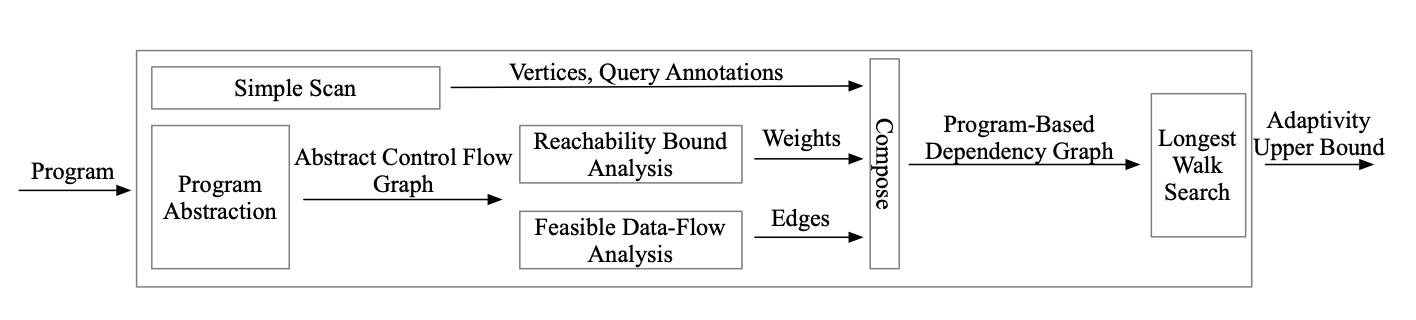
\includegraphics[width=1.0\columnwidth]{adapfun.png}
  \vspace{-0.3cm}
  \caption{The overview of {\THESYSTEM}}
  \label{fig:adaptfun}
  \vspace{-0.5cm}
\end{figure}
%
Below is the outline of the {\THESYSTEM}.
% through Section~\ref{sec:alg_vertexgen}, Section~\ref{sec:alg_weightedgegen} and~\ref{sec:alg_graphgen}:
\begin{enumerate}
  \item \textbf{Graph Estimation}
  Because adaptivity is defined over a program's \emph{quantitative dependency graph} (in Definition~\ref{def:trace_graph}),
  this algorithm first estimates this graph for the program statically
  in Section~\ref{sec:alg_graphgen}.
  % execution-based dependency graph (in Definition~\ref{def:trace_graph})
  % Execution-Based Dependency Graph (in Definition~\ref{def:trace_graph}). 
  It estimates the four components of this graph in two steps and then composes them into an estimated dependency graph
  %  for a program 
  in the last step.
  %  Firvertices, edges, and the weight of every node, as well as some annotations which marks the query usage. 
  % The algorithm is presented in Section~\ref{sec:alg_graphgen} as follows.
  The steps are summarized  as follows.
\begin{enumerate}
  \item \textbf{Vertex and Query Annotation Estimation}
  Vertices and query annotations in this graph are the assigned variables with unique labels. These are extracted directly from the program as in Section~\ref{sec:alg_vertexgen}.
  \item \textbf{Edge and Weight Estimation}
  \\
  This step estimates the edge and weight for a quantitative dependency graph. It combines the control, data-flow  analysis algorithm and the loop bound inference algorithm.
  There are three computation steps in this algorithm.
  \\
  \textbf{Abstract Control Flow Graph.}
  In order to perform the dependency analysis and quantitative analysis, this step first generates an \emph{abstract control flow graph} for a program in Section~\ref{sec:abscfg}.
  \\
  \textbf{Edges Estimation via Combined Flow Analysis.} 
  The step is presented in
  Section~\ref{sec:alg_edgegen}. It performs over the \emph{abstract control flow graph}, which combines both control flow and data flow analysis.
  It estimates the \emph{dependency relation} between each pair of the labeled variables in a program by considering both the control flow and data flow.
  Then it uses the estimated dependency relation to approximate the edge
  %  of the quantitative dependency graph 
  between each pair of vertices.
  \\
  \textbf{Weights Estimation via Quantitative Analysis.} 
  This step is presented in Section~\ref{sec:alg_weightgen}. 
  It performs over the same \emph{abstract control flow graph} and computes the upper bound on the maximal visiting times of each labeled variable for a program.
  %  can be visited during execution. 
  % It performs over the same \emph{abstract control flow graph} as well. 
  It estimates the reachability bound for every vertex over the \emph{abstract control flow graph},
  and this reachability bound is used to estimate the maximal visiting times of each labeled variable in a program and the weight of the corresponding vertex.
  %  of this quantitative dependency graph.
\item  \textbf{Graph Estimation.} 
In Section~\ref{sec:alg_graphgen}, we construct the final approximated graph,
named \emph{program-based dependency graph} by simply composing the four estimated ingredients. 
Overall, this \emph{program-based dependency graph} has a similar topology structure as 
the \emph{execution-based dependency graph}. It has the same
vertices and query annotations, but approximated edges and weights. 
% The edge between vertices considers both control flow and data flow, See
% Section~\ref{sec:alg_edgegen}
% \item Every vertex and edge come with a weight, which tells the maximal times each vertex and edge can be visited in realistic execution. This weight is estimated by a reachability bound analysis on each vertex, See Section~\ref{sec:alg_weightgen}.
% % \item Each edge also vertices co
\end{enumerate}

\item \textbf{Adaptivity Computation.} 
Likewise the adaptivity in Definition~\ref{def:trace_adapt},
%  is defined as a finite walk in the \emph{execution based dependency graph}, 
the static estimation on the \emph{adaptivity} also relies on finding a walk in the \emph{program-based dependency graph}.  
% The construction of the stastic analysis dependency graph is of great value of showing some useful properties of the target program, such as dependency between variables, the execution upper bound of a certian command, while the key novelty is our path searching algorithm, which connects all the information we need in the static anlaysis dependency graph and provides us a sound over-estimation of adaptivity! In order to get a sound but precise upper bound,
We discuss some challenges in finding the 'appropriate' walk in the graph, and how our algorithm responds to these challenges as
% . We present the path searching algorithm 
in Section~\ref{sec:alg_adaptcompute}.
% % Section~\ref{sec:alg_edgegen}
% \item  Finally, with all the ingredients ready, we construct the final approximated program-based dependency graph in Section~\ref{sec:alg_graphgen}
\end{enumerate}

\subsection{Vertex and Query Annotation Estimation}
\label{sec:alg_vertexgen}
\paragraph{Vertex Estimation}
The first component of the \emph{program-based dependency graph} is the vertex set, which is identical to the 
\emph{execution-based dependency graph}.
% of every vertex in the static analysis dependency graph are actually identical as the  Execution-Based Dependency Graph, 
Every vertex is an assigned variable in the program, which comes from an assignment command or query request command with a unique label. 
These vertices are collected by statically scanning the program, like what we do for vertices of the \emph{execution-based dependency graph}, as follows.
%
\highlight{
\[
    \progV(c) \triangleq \left\{ 
  x^l \in \mathcal{LV}
  ~ \middle\vert ~
  x^l \in \lvar(c)
  \right\}
  \]
  }
  %
where $\mathcal{A}_{\lin}$ is the set of arithmetic expressions over $\mathbb{N}$ and program's input variables. 

\paragraph{Query Annotation Computation}
The static scanning of the programs also tells us whether one vertex(assigned variable) is assigned by a query request.
% We have similar definition when defining the Execution-Based Dependency Graph, 
Identically to the 
\emph{execution-based dependency graph}, $\progF(c)$ is
a set of pairs $\progF(c) \in \mathcal{P}(\mathcal{LV} \times \{0, 1\} )$ 
% is the set of pairs 
% The weight for each vertex in $\progV(c)$ is computed 
mapping each $x^l \in \progV(c)$ to either $0$ or $1$. 
$1$ denotes $x^{l}$ is a member of $ \qvar_{c}$, which is the set of program's variables assigned with query requests, 
and $0$ means $x^{l}$ not in this set. 
It is defined formally below.
%
\[\progF(c) =\left\{(x^l, n)  \in  \mathcal{LV} \times \{0, 1\} 
~ \middle\vert ~
x^l \in \lvar_{c},
n = 1 \iff x^l \in \qvar_{c} \land n = 0 \iff  x^l \not\in \qvar_{c} .
\right\}\]

\subsection{Edge and Weight Estimation}
\label{sec:alg_weightedgegen}
The edges and weight are estimated through a combined control, data flow, and loop bound analysis.
Because these analyses are all performed on basis of the \emph{Abstract Transition Graph} of the program, we first introduce how to generate this \emph{abstract transition graph} in Section~\ref{sec:abscfg}.
Then Section~\ref{sec:alg_edgegen} presents the edge estimation based on a combined control and data flow analysis algorithm,
and Section~\ref{sec:alg_weightgen}
computes the weight through a loop bound analysis.

\subsubsection{Abstract Execution Control Flow graph}
\label{sec:abscfg}
This section shows how to generate the abstract transition graph $\absG(c)$ of a
program $c$ through constructing its vertices and edges.

An \emph{Abstract Transition Graph}, $\absG(c)$ for a program $c$ is composed of
a vertex set $\absV(c)$ and an edge set $\absE(c)$, $\absG(c) \triangleq (\absV(c), \absE(c))$.
% For a program $c$, this analysis first generates its abstract execution control flow graph notated as follows,
% \[\absG(c) =(\absV(c), \absE(c))\]
%
\\
Every 
vertex $l \in \absV(c)$ is the label of a labeled command in $c$, which is unique.
We also call the unique label as program point.
% corresponds to a program point $l$, which is a unique
% label of a command in this program.
% $\absV(c)$ is the set of $c$'s all program points,
\\
Each edge $(l \xrightarrow{dc} l') \in \absE(c)$ is an abstract transition
between two program points $l, l'$. 
There is an edge from $l$ to $l'$ if and only if
the command with label $l'$ can execute right after the execution of the command with label $l$.
% if and only if there is a control flow between two program points.
Each edge is annotated by a constraint $dc \in \dcdom^{\top}$, which is generated from the command with label $l$.
This constraint describes the abstract execution of the command with $l$. 
%  before the introduction of the edge and weight estimation.  
% We discuss the vertices and edge of the
% abstract transition graph for a program $c$, $\absG(c)$.

\paragraph{Abstract Control Flow Graph Vertices Construction}
\label{sec:abscfg-vertex}
Every 
vertex $l \in \absV(c)$ corresponds to a program point $l$, which is a unique
label of a command in this program.
Concretely,
the vertices of this graph is the set of $c$'s labels with the exit label ${\lex}$ formally as follows,
\[ 
  \absV(c) = \lvar(c)\cup\{{\lex}\}
\]
%  corresponding to a label command in the program.

\paragraph{Abstract Control Flow Graph Edge Construction}
\label{sec:abscfg-edge}
Each edge $(l \xrightarrow{dc} l') \in \absE(c)$ is an abstract transition
between two program points $l, l'$. 
There is an edge from $l$ to $l'$ if and only if
the command with label $l'$ can execute right after the execution of the command with label $l$.
% if and only if there is a control flow between two program points.
Each edge is annotated by a constraint $dc \in \dcdom^{\top}$ generated from the command with label $l$.
This constraint describes the abstract execution of the command with $l$. 
This step shows how to generate the abstract transition graph $\absG(c)$ of a
program $c$ through constructing its vertices and edges.
\\
  The vertices can be easily collected and the key point of the abstract
  transition graph for a program is constructing the edge set, $\absE(c)$ for a program $c$.
  It relies on the control flow analysis and the program abstraction of each command.
  %  and abstract transition (we also call it abstract event).
  To make it easy to understand, it
  is an enriched control flow graph with an annotation on each edge.
  The edge set is constructed by a program abstraction method in three steps.
  \\
  In the first step, \textbf{Constraint Computation} generates a constraint
  over the expression for every program's labeled command,
  which is used as the annotation of an edge.
  \\
  In the second step, \textbf{Initial and Final State Computation} generates two sets for each command. 
  The initial state is a set that contains the
  program point where this command \todo{starts} executing, 
  and the final state is a set
  that contains the constraint of this command
  and the continuation program points after the execution of this command.
  \\ 
  In the third step, \textbf{Abstract Event Computation} generates a set of edges for the program.
  Each edge is a pair of initial and finial state.
  % The annotation of each edge is a constraint generated by a program abstraction method.
  % by adopting the program abstraction.
  %  method in Section 6 in~\cite{sinn2017complexity}.
  %  the program's every command.
% It is computed as follows.
  % The edge in the abstract transition graph comes from the abstract execution trace of the program. 
  % The abstract execution trace, an abstract representation of the execution, consists of a set of abstract events. 
%   The edge in the abstract transition graph comes from the program's abstract events set $\absflow(c)$.
%   Each abstract event $(l_1, dc, l_2)$ in this set represents an edge in $\absE(c)$.
%   % Then, every abstract transition in the abstraction execution trace corresponds to an edge in the abstract transition graph. In another word, the edge $(l_1, dc, l_2)$ in the abstract transition graph, represents an abstract transition 
% %  from $l_1$ to $l_2$, with a set of difference constraints $dc$. 
%  Also notice, the difference constraints generated during the abstract transition appears in the edge as annotation.
%
\paragraph{Constraint Computation}
In this step, we first show how to compute the constraints for expressions in a program $c$,
by a program abstraction method adopted from the
algorithm in Section 6 in~\cite{sinn2017complexity}.
\\
Given a program $c$,
every expression in an assignment command or in the guard of a $\eif$ or $\ewhile$ command
is transformed into a constraint.

\highlight{Notations / Formal Definitions:}
\begin{itemize}
\item Operator: $\absexpr : \mathcal{A} \cup \mathcal{B} \to DC(\mathcal{VAR}  \cup \constdom)\cup \booldom \cup \{\top\}$
%
\item Constrains, $\dcdom^{\top}$ is composed of the \emph{Difference Constraints} $DC(\mathcal{VAR}  \cup \constdom)$, the \emph{Boolean Expressions} $\booldom$ and $\top$.
%
\begin{itemize}
\item The difference constraints $DC(\mathcal{VAR}  \cup \constdom)$ is the set of all the inequality of
form $x' \leq y + v$ where $x \in \mathcal{VAR} $, 
$y \in \mathcal{VAR}$ and $v \in \constdom$.
The \emph{Symbolic Constant} set $\constdom = \mathbb{N} \cup \inpvar \cup{\infty \cup{Q_m}}$
is the set of natural numbers with $\infty$, the input variables, and a symbol $Q_m$ representing the abstract value of a query request.
An inequality $x' \leq y + v$ describes that the value of $x$ in the current state is
at most the value of $y$ in the previous state plus some constant $v$.
When a difference constrain shows up as an edge annotation, $l \xrightarrow{x' \leq y + v} l'$,
% Then $x'$ 
it denotes that
the value of variable $x$
after executing the command at $l$ is at most
% and the right-hand side describes 
the value of variable $y$ plus $v$ before the execution.
For every expression in each of the label command, it is computed in three steps via program abstraction method adopted from the Section~6 in \cite{sinn2017complexity}. 
%
\item The Boolean Expressions $b$ from the set $\booldom$.
$b$ on an edge $l \xrightarrow{b} l'$ describes
that after evaluating the guard with label $l$,
$b$ holds and the command with label $l$ will execute right after.
%
\item The top constraint, $\top$ denotes true. It is preserved for $\eskip$ command.
%
\end{itemize}
\end{itemize}

\highlight{Computation Steps:}
\begin{defn}[Constraint Computation]
  \label{def:constraint_compute}
  For a program $c$, a boolean expression $\bexpr$ in the guard of a $\eif$ or $\ewhile$ command
  or an expression $\expr$ and a variable $x$
  in an assignment command $\assign{x}{\expr}$,
  % or 
  % For a boolean expression $\bexpr$ or an arithmetic expression $\aexpr$ and a variable $x$,
  the constraint $\absexpr(\bexpr, \_)$ or $\absexpr(x - v, x)$ is computed as follows,
  \[
    \begin{array}{ll} 
      \absexpr(x - v, x)  = x' \leq x - v  & x \in \grdvar \land v \in \mathbb{N} \\
      \absexpr(y + v, x)  = x' \leq y + v  & x \in \grdvar \land v \in \mathbb{Z} \land y \in (\grdvar \cup \constdom) \\
      \absexpr(v, x)  = x' \leq v + 0  & x \in \grdvar \land v \in (\grdvar \cup \constdom) \\
      \absexpr(y + v, x)  = x' \leq y + v & \\
      \grdvar = \grdvar \cup \{y\} & x \in \grdvar \land v \in \mathbb{Z} \land y \notin (\grdvar \cup \constdom)  \\
      \absexpr(\qexpr, x)  = x' \leq 0 + Q_m & x \in \grdvar \land \qexpr \text{ is a query expression}  \\
      \absexpr(\expr, x) = x' \leq \infty  &  x \in \grdvar \land \expr \text{ doesn't have any of the forms as above} \\
      % \absexpr(\qexpr, x)  = x' \leq 0 + Q_m & x \in \grdvar \land \qexpr \text{ is a query expression}  \\
      \absexpr(\expr, x) = \etrue  &  x \notin \grdvar \\
      \absexpr(\bexpr, \_) = \bexpr   & \\
      % \absexpr(y + v, x)  = x' \leq y + v & \\
      \grdvar = \grdvar \cup FV(\bexpr) &  x \in \grdvar \land \bexpr \text{ is a boolean expression} \\
    \end{array}
    \]
  \end{defn}
%
  $\grdvar$ is the set of variables used in the guard expression of every while command in the program $c$. 
  In the case 4, if a variable $x$, belonging to the set 
  $\grdvar$ is updated by a variable $y$, which isn't in this set, 
  we add $y$ into the set $\grdvar$ and repeat 
  above procedure  until $\grdvar$ and $\absexpr(\expr, x)$ is stabilized. 
  % \wq{I do not understand this sentence:-(}
  \\
Specifically 
% understanding the intuition, 
we handle a 
% simplified 
normalized expression, $x > 0$
in guards of while loop headers, and 
%  \wq{I do not understand this sentence:-(}
%  .
% \\
% The counter variables only increase, decrease or reset by expression in the form of arithmetic minus and plus (able to extend to max and min.)
the counter variable $x$ only increase, decrease or reset by 
% expression in the form of 
simple arithmetic expression (mainly multiplication, division, minus and plus (able to extend to max and min)). 
The counter variable $x$ is generalized into norm when the boolean expression $x > 0$
in $\ewhile$ doesn't have the form $x > 0$.
The way of normalizing the guards and computing the norms is adopted from the computation step 1 in Section 6.1 in paper \cite{sinn2017complexity}. 
% \\
% For more complex expression assignments, where the counter reset, or calculated from $\elog$, 
% multiplication or division, and expressions involving multiple variables, the constraint is approximated as reset of $\infty$.
% \\
% % This simplification \wq{which part we simplify here?} 
% This approximation strategy
% doesn't affect our analysis results in our examples. It is easy to extend the normalized expression 
% into more complex forms as in \cite{sinn2017complexity}, as well as the 
% counter variable manipulation with more advanced expressions.
% \\ 
% The boolean expression in the guard of $\ewhile$ command is normalized into form of $ x > 0$ where $x^l \in \lvar_c$ for some $l$.
\begin{defn}[Symbolic Expression ($\mathcal{A}_{S}$)]
  $\mathcal{A}_{S}$ is the set of all the symbolic expressions 
over $\constdom$.
% For concise, $\mathcal{A}_{\lin}$ is used as the same meaning of $\mathcal{A}_{\lin}$ in the follows, to denote the arithmetic expression 
% over the symbolic variables, (i.e., $\mathbb{N}$ with input variables).
\end{defn}
The symbolic expression set is a subset of arithmetic expressions over $\mathbb{N}$ with input variables, 
i.e., $\mathcal{A}_{S} \subseteq \mathcal{A}_{\lin}$.
% \subsubsection{Abstract Transition Graph through an Example}
\paragraph{Abstract Initial and Final State Computation}
This step computes two sets for each command. 
The initial state is a set that contains the
program points before executing this command, which is computed by the standard initial state generation method from control flow analysis.
The final state is a set
that contains the constraint of this command and the program points after the execution of this command.
This set is enriched 
% program's initial and final states 
from the standard control flow analysis.

%
\highlight{Notations / Formal Definitions:}
\begin{itemize}
\item The abstract initial state: $\absinit(c) \in \ldom$.
%
\item The abstract Final State: $\absfinal(c) \in \mathcal{P}(\ldom \times \dcdom^{\top})$
\end{itemize}

\highlight{Computation Steps:}
\begin{itemize}
  \item The \emph{abstract initial state}, $\absinit(c) \in \mathcal{P}(\ldom)$
  for a command $c$ is the set of the initial program points.
Each point in this set is a unique program label corresponds to the command before executing this command. 
% when executing this program.
\\
Given a program $c$, its abstract initial state, $\absinit(c)$ is computed as follows,
%
\[
  \begin{array}{ll}
    \absinit(\clabel{\assign{x}{\expr}}{}^l)  & = \{l\}  \\
    \absinit(\clabel{\assign{x}{\query(\qexpr)}}{}^l)  & = \{l\} \\
    \absinit(\clabel{\eskip}^{l})  & = l \\
    \absinit(\eif [b]^l \ethen c_1 \eelse c_2)  & = \{l\} \\
    \absinit(\ewhile [b]^l \edo c)  & = \{l\} \\
    \absinit(c_1 ; c_2)  & = \absinit(c_1) \\
 \end{array}
 \]
%
%
\item The \emph{abstract final state} of the program $c$, 
$\absfinal(c) \in \mathcal{P}(\ldom \times \dcdom^{\top})$
is a set of pairs, $(l, dc)$ with a
program point (i.e., a label), $l$ as the first component and a constraint, 
$dc$ as the second component.
% Every pair in $\absfinal(c)$ 
The program point $l$ corresponds to the labeled command after the execution of $c$,
and the constraint $dc$ in this pair is computed by $\absexpr$ for the expression in $c$.
%  in the first step.
\\
Given a program $c$, its final state, $\absfinal(c)$ is computed as follows,
% $\absfinal(c) \in\mathcal{P}(\ldom \times \dcdom^{\top})$,
% computes the set of Abstract Final State for the command. 
 \[
  \begin{array}{ll}
    \absfinal(\clabel{\assign{x}{\expr}}{}^l)  & = \{(l, \absexpr\eapp (\expr, x))\}  \\
     \absfinal(\clabel{\assign{x}{\query(\qexpr)}}{}^l)  & = \{
      (l, x' \leq 0 + Q_m )\}  \\
     \absfinal(\clabel{\eskip}^{l})  
     & = \{(l, \top)\} \\
     \absfinal(\eif [b]^l \ethen c_1 \eelse c_2)  & = \absfinal(c_1) \cup \absfinal(c_2) \\
     \absfinal(\ewhile [b]^l \edo c)  & = \{(l, \absexpr(\bexpr, \top))\} \\
     \absfinal(c_1 ; c_2)  & =  \absfinal(c_2) \\
 \end{array}
 \]
 %
\end{itemize}
 \paragraph{Abstract Event Computation} Each abstract event is an edge between two vertices in the abstract transition graph.
 It is generated by computing the initial state and finial state interactively and recursively for a program $c$.
 
 \highlight{Notations / Formal Definitions:}
 \begin{itemize}
  \item \emph{Abstract Event}: 
  $\absevent \in $
  $\ldom \times \dcdom^{\top} \times \ldom$
  \item \emph{Abstract Event Computation}: $\absflow \in \cdom \to \mathcal{P}( \ldom \times \dcdom^{\top} \times \ldom )$
 \end{itemize}
 Its type is defined as follows,
 \begin{defn}[Abstract Event]
   \label{def:abs_event}
   Abstract Event: 
   $\absevent \in $
   $\ldom \times \dcdom^{\top} \times \ldom$
   is a 
   % pair of abstract initial state and final state.
   triple where the first and third components are labels,
   second component is a constraint from $\dcdom^{\top}$.
   % the thrid % computed from program's abstract final and initial state, $\absfinal(c)$ and $\absinit(c)$ with formal definition, and algorithm detail in Appendix.
   %  the constraint and the third corresponds to a final state.
   \end{defn}
   In an abstract event $(l, dc, l')$ of a program $c$, 
   the first label $l \in \ldom$ corresponds to an initial state of $c$, and 
   the second label $l' \in \ldom$ with the constraint $dc \in \dcdom^{\top}$ correspond to an abstract final state of $c$.
  The abstract initial state is a label from $\ldom$.
%  The abstract final state is a pair from $\ldom \times \dcdom^{\top}$,  
%  where first component is a label from $\ldom$ and the second component is a constraint from $\dcdom^{\top}$.
 %
We abuse the notation $\mathcal{P}(\absevent)$ for the power set of all abstract events.

 \highlight{Computation Steps:}
\\
% The abstract event is computed for w.r.t the program in Definition~\ref{def:absevent_compute}, 
%  generated during computing its abstract execution trace, 
%  , and we have $\absflow(c) \in \mathcal{P}(\absevent)$.
%  Now, we  extract the abstract execution trace  $\absflow(c)$ for a program, which computes the 
%  The \emph{Abstract Execution Trace} for program $c$ is a s
The set of the abstract events $\absflow(c)$ for a program $c$
% .
%  Its type is formally defined 
is computed as follows in Definition~\ref{def:absevent_compute}.
 %
 \begin{defn}[Abstract Event Computation]
 \label{def:absevent_compute}
  $\absflow \in \cdom \to \mathcal{P}( \ldom \times \dcdom^{\top} \times \ldom )$
  \end{defn}
 %
%  The \emph{Abstract Execution Trace} for program $c$ is computed as follows.
%  \\
  % We now show how to compute the abstract execution trace. 
 We first append a $\eskip$ command with 
%  a symbolic label $l_e$, i.e., $\clabel{\eskip}^{l_e}$ at the end of the program $c$, and compute the $\absflow(c) = \absflow'(c')$ for $c'$, where $c' = c;\clabel{\eskip}^{l_e}$ as follows,
the label $\lex$, i.e., $\clabel{\eskip}^{l_{ex}}$ at the end of the program $c$, and construct 
the program $c' = c;\clabel{\eskip}^{l_{ex}}$.
Then, we compute the $\absflow(c) = \absflow'(c')$ for $c'$ as follows,
 %
 {\footnotesize
 \[
   \begin{array}{ll}
      \absflow'(\clabel{\assign{x}{\expr}}{}^l)  & = \emptyset  \\
      \absflow'(\clabel{\assign{x}{\query(\qexpr)}}{}^l)  & = \emptyset  \\
      \absflow'([\eskip]^{l})  & = \emptyset \\
      \absflow'(\eif [b]^l \ethen c_t \eelse c_f)  & =  \absflow'(c_t) \cup \absflow'(c_f)
        \\ & \quad 
        \cup \{(l, \absexpr(\bexpr, \top),  \absinit(c_t) ) ,  (l, \absexpr(\neg\bexpr, \top), \absinit(c_f)) \} \\
       \absflow'(\ewhile [b]^l \edo c_w)  & =  \absflow'(c_w) \cup \{(l, \absexpr(\bexpr, \top), \absinit(c_w)) \} 
       \\ & \quad 
       \cup \{(l', dc, l)| (l', dc) \in \absfinal(c_w) \} \\
       \absflow'(c_1 ; c_2)  & = \absflow'(c_1) \cup  \absflow'(c_2) 
       \\ & \quad 
       \cup \{ (l, dc, \absinit(c_2)) | (l, dc) \in \absfinal(c_1) \} \\
   \end{array}
   \]
   }
   Notice $\absflow'([x := \expr]^{l})$, $\absflow'([x := \query(\qexpr)]^{l})$ and $\absflow'([\eskip]^{l})$ are all empty set. 
   For every event $\event$ with label $l$ in an execution trace $\trace$ of program $c$, 
   there is an abstract event in program's abstract execution trace of form $(l, \_, \_)$.  
   We also show the soundness of the abstract events computation in Appendix.

 \highlight{Theorem Guarantee:}
   \begin{lem}[Soundness of the Abstract Events Computation]
     \label{lem:abscfg_sound}
     For every program $c$ and
     an execution trace $\trace \in \mathcal{T}$ that is generated w.r.t.
     an initial trace  $\vtrace_0 \in \mathcal{T}_0(c)$,
     there is an abstract event $\absevent = (l, \_, \_) \in \absflow(c)$ 
     % with initial label $l$
     for every event $\event \in \trace$ having the label $l$, i.e., $\event = (\_, l, \_, \_)$.
      %
   \[
     \begin{array}{l}
       \forall c \in \cdom, \vtrace_0 \in \mathcal{T}_0(c), \trace \in \mathcal{T} ,  \event = (\_, l, \_, \_) \in \eventset \st
   \config{{c}, \trace_0} \to^{*} \config{\eskip, \trace_0 \tracecat \vtrace} 
   \land \event \in \trace 
   \\
   \qquad \implies \exists \absevent = (l, \_, \_) \in (\ldom\times \dcdom^{\top} \times \ldom) \st 
   \absevent \in \absflow(c)
   \end{array}
   \]
   \end{lem}
%    This lemma is proved formally in Appendix~\ref{apdx:rb_soundness}.
% For every event $\event$ with label $l$ in an execution trace $\trace$ of program $c$, 
% there is an abstract event in program's abstract events computation of form $(l, \_, \_)$. 
This lemma is proved formally in Appendix~\ref{apdx:reachability_soundness}.
\\
For every program point $l$ corresponding to an assignment command in a program $c$,
%  $x^l \in \lvar_c$, 
there is a unique abstract event in the program's abstract events set $\absevent \in \absflow(c)$ of form $(l, \_, \_)$. 
\begin{lem}[Uniqueness of the Abstract Events Computation]
  \label{lem:abscfg_uniquex}
  For every program $c$ and
  an execution trace $\trace \in \mathcal{T}$ that is generated w.r.t.
  an initial trace  $\vtrace_0 \in \mathcal{T}_0(c)$,
  there is a unique abstract event $\absevent = (l, \_, \_) \in \absflow(c)$ 
  % with initial label $l$
  for every assignment event $\event \in \eventset^{\asn}$ in the
  execution trace having the label $l$, i.e., $\event = (\_, l, \_, \_)$ and  $\event \in \trace$.
%
\[
  \begin{array}{l}
    \forall c \in \cdom, \vtrace_0 \in \mathcal{T}_0(c), \trace \in \mathcal{T} ,  \event = (\_, l, \_) \in \eventset^{\asn} \st
\config{{c}, \trace_0} \to^{*} \config{\eskip, \trace_0 \tracecat \vtrace} 
\land \event \in \trace 
\\
\qquad \implies \exists! \absevent = (l, \_, \_) \in (\ldom\times \dcdom^{\top} \times \ldom) \st 
\absevent \in \absflow(c)
\end{array}
\]
\end{lem}
This lemma and proof is also 
formalized in Appendix~\ref{apdx:reachability_soundness}.

  \paragraph{Edge Construction}
The edge for $c$'s abstract transition graph is constructed simply by computing the program's abstract events set, $\absflow(c)$ as follows,
  \[
    \absE(c) = \{(l_1, dc, l_2) | (l_1, dc, l_2) \in \absflow(c)\}
  \]
% The edge set is constructed simply by computing the program's abstract events set, $\absflow(c)$.
%   Each abstract event $(l_1, dc, l_2)$ in this set represents an edge in $\absE(c)$.
%   % Then, every abstract transition in the abstraction execution trace corresponds to an edge in the abstract transition graph. In another word, the edge $(l_1, dc, l_2)$ in the abstract transition graph, represents an abstract transition 
% %  from $l_1$ to $l_2$, with a set of difference constraints $dc$. 
%  The constraints generated in the abstract event appears in the edge as annotation.
% We have a pre-processing algorithm to go through the programs and returns the list of labels associating with a loop and whose visiting times need to be analyzed.
%
\paragraph{Abstract Transition Graph Construction} 
With the vertices $\absV(c)$ and edges $\absE(c)$ ready, we construct the abstract transition graph, formally in
% Through a program $c$'s abstract events computation, its abstract transition graph is computed in 
Definition~\ref{def:abs_cfg}.
%
\begin{defn}[Abstract Transition Graph]
\label{def:abs_cfg}
Given a program $c$, 
its \emph{abstract transition graph} $\absG(c) =(\absV(c), \absE(c))$ is computed as follows,
\\
$\absE(c) = \{(l_1, dc, l_2) | (l_1, dc, l_2) \in \absflow(c)\}$,
\\
$\absV(c) = \lvar(c)\cup\{\lex\}$
% \\
%  $\absW(c) 
% \triangleq \left\{ (l, w) \in \mathbb{L} \times \mathcal{A}_{\lin} \right\}$.
\end{defn}
\paragraph*{Example}
%
The edge $(0 \xrightarrow{a' \leq 0} 1)$ on the top, tells us the command 
$\clabel{\assign{a}{0}}^0$ is executed with a continuation point $1$ such that the
% where the 
command $\clabel{\assign{j}{k}}^1$ will be executed next.
The annotation $a' \leq 0$ is a difference constraint 
computed for
% by abstracting
the expression $0$ in the assignment command $\assign{a}{0}$.
%  from the function $\absexpr(0)$.
It represents that the value of $a$ is less than or equal to $0$ after the
execution of $\clabel{\assign{a}{0}}^0$ and before executing $\clabel{\assign{j}{k}}^1$.
Another example edge $5 \xrightarrow{a' \leq a + x } 2$ describes the execution of
 the command at line $5$
$\clabel{\assign{a}{x + a}}^{5}$.
This edge has difference constraint $a' \leq a+x $.
The $a'$ on the left side of $a' \leq a+x$ represents the value of $a$ after executing this assignment command.
The boolean constraint $j \leq 0 $ on the edge $2 \xrightarrow{j \leq 0} 6$
represents the negation of the testing guard $j > 0$
in the $\ewhile$ command with loop header at line $2$.
The edge from $3$ to $4$ comes from a query request command.
The constraint over this edge, $x' < Q_m$ describes after executing the query request command,
$\clabel{\assign{x}{\query(\chi[j])} }^{3}$, the query request results stored in $x$ is bounded by $Q_m$. 

\begin{figure} 
    \centering
    \begin{subfigure}{.2\textwidth}
    \begin{centering}
    {\small
    $
        \begin{array}{l}
              \clabel{ \assign{a}{0}}^{0} ;   
                \clabel{\assign{j}{k} }^{1} ; \\
                \ewhile ~ \clabel{j > 0}^{2} ~ \edo ~ \\
                \Big(
                 \clabel{\assign{x}{\query(\chi[j])} }^{3}  ; \\
                 \clabel{\assign{j}{j-1}}^{4} ;\\
                \clabel{\assign{a}{x + a}}^{5}       \Big);\\
                \clabel{\assign{l}{\query(\chi[k]*a)} }^{6}\\
            \end{array}
    $
    }
    \caption{}
    \end{centering}
    \end{subfigure}
    \begin{subfigure}{.38\textwidth}
        \begin{centering}
      \begin{tikzpicture}[scale=\textwidth/20cm,samples=200]
      \draw[] (-7, 10) circle (0pt) node{{ $0$}};
      \draw[] (0, 10) circle (0pt) node{{ $1$}};
      \draw[] (0, 7) circle (0pt) node{\textbf{$2$}};
      \draw[] (0, 4) circle (0pt) node{{ $3$}};
      \draw[] (0, 1) circle (0pt) node{{ $4$}};
      \draw[] (-7, 1) circle (0pt) node{{ $5$}};
      % Counter Variables
      \draw[] (6, 7) circle (0pt) node {\textbf{$6$}};
      \draw[] (6, 4) circle (0pt) node {{ $\lex$}};
      %
      % Control Flow Edges:
      \draw[ thick, -latex] (-6, 10)  -- node [above] {$a' \leq 0$}(-0.5, 10);
      \draw[ thick, -latex] (0, 9.5)  -- node [left] {$j' \leq k$} (0, 7.5) ;
      \draw[ thick, -latex] (0, 6.5)  -- node [right] {$j > 0$}  (0, 4.5);
      \draw[ thick, -latex] (0, 3.5)  -- node [right] {$x' \leq Q_m$} (0, 1.5) ;
      \draw[ thick, -latex] (-0.5, 1)  -- node [above] {$j' \leq j - 1$} (-6, 1) ;
      \draw[ thick, -latex] (-6, 1.5)  -- node [left] {$a' \leq x + a$} (-0.5, 7)  ;
      \draw[ thick, -latex] (0.5, 7)  -- node [above] {$ j \leq 0 $}  (5.5, 7);
      \draw[ thick, -latex] (6, 6.5)  -- node [right] {$l' \leq k * a$} (6, 4.5) ;
      \end{tikzpicture}
      \caption{}
        \end{centering}
        \end{subfigure}
        \begin{subfigure}{.38\textwidth}
          \begin{centering}
        %   \todo{abstract-cfg for two round}
        \begin{tikzpicture}[scale=\textwidth/20cm,samples=200]
        \draw[] (-10, 10) circle (0pt) node{{ $0: 1$}};
        \draw[] (0, 10) circle (0pt) node{{ $1: 1$}};
        \draw[] (0, 7) circle (0pt) node{\textbf{$2: k$}};
        \draw[] (0, 4) circle (0pt) node{{ $3: k$}};
        \draw[] (0, 1) circle (0pt) node{{ $4: k$}};
        \draw[] (-10, 1) circle (0pt) node{{ $5: k$}};
        % Counter Variables
        \draw[] (6, 7) circle (0pt) node {\textbf{$6: 1$}};
        \draw[] (6, 4) circle (0pt) node {{ $\lex: 1$}};
        %
        % Control Flow Edges:
      \draw[ thick, -latex] (-8, 10)  -- node [above] {$a' \leq 0$}(-1.5, 10);
      \draw[ thick, -latex] (0, 9.5)  -- node [left] {$j' \leq k$} (0, 7.5) ;
      \draw[ thick, -latex] (0, 6.5)  -- node [right] {$j > 0 $}  (0, 4.5);
      \draw[ thick, -latex] (0, 3.5)  -- node [right] {$x' \leq Q_m$} (0, 1.5) ;
      \draw[ thick, -latex] (-1.5, 1)  -- node [above] {$j' \leq j - 1$} (-8, 1) ;
      \draw[ thick, -latex] (-8, 1.5)  -- node [left] {$a' \leq x + a$} (-1.5, 7)  ;
      \draw[ thick, -latex] (1.5, 7)  -- node [above] {$j \leq 0 $}  (4.5, 7);
      \draw[ thick, -latex] (6, 6.5)  -- node [right] {$l' \leq k * a$} (6, 4.5) ;
        \end{tikzpicture}
        \caption{}
          \end{centering}
          \end{subfigure}
      \caption{(a) The same $\kw{towRounds(k)}$ program as Figure~\ref{fig:overview-example}
      (b) The abstract control flow graph for $\kw{towRounds(k)}$  (c) The abstract control flow graph with the reachability bound for $\kw{towRounds(k)}$.}
      \label{fig:abscfg_tworound}
    \end{figure}
%

\subsubsection{Edge Estimation via Dependency Analysis Algorithm}
\label{sec:alg_edgegen}
Since the edges of the execution-based graph of a program relies on the dependency relation, it contains both control flow and data flow. 
In this sense, We first develop a \emph{feasible data-flow} relation to estimate the data dependency relation, which catches these two flows.
Then we construct the edges for $\progG(c)$ based on this \emph{feasible data-flow} relation.
%  of our static analysis dependency graph also covers these two kind of flows. 
This algorithm named Feasible Data-Flow Generation. It 
considers both the control flow and data flow and
is a sound approximation of the edges in the execution based dependency graph.
The three steps in this algorithm is summarized as follows,
\begin{enumerate}
  \item The \textbf{Reaching Definition} analysis computes a set of labeled variables, $\live(l, c)$ for every label $l$ in $c$
  over its abstract control flow graph, $\absG(c)$.
  The computation performs the standard reaching definition analysis and working-list algorithm over the abstract control flow graph, $\absG(c)$. 
  % as $\live(l, c)$ for every label $l$ in a program $c$. 
  $\live(l, c)$ contains all the labeled variables which are reachable at program point $l$. 
  % The computation details for $\live(l, c)$ are standard and omitted here, they can be found in Appendix.
  \item The \textbf{Feasible Data-Flow} computation combines the $\live(l, c)$, $\absG(c)$ and data flow analysis. 
  It computes the \emph{feasible data-flow} relation,
  % estimates the data dependency relation, 
  $\flowsto(x^i, y^j, c)$ for each pair of the $c$'s labeled variables, $x^i, y^j \in \lvar(c)$ in Definition~\ref{def:feasible_flowsto}. $\flowsto(x^i, y^j, c)$ is a sound approximation 
  of the \emph{variable may-dependency} relation, $\vardep(x^i, y^j, c)$ for every $x^i, y^j \in \lvar(c)$.
  %  over labeled variables for every program.
  The formal proof is in the Appendix. We also discuss that the combined analysis gives more precise approximation on the \emph{data may-dependency} than single analysis in Appendix.
\item \textbf{Edge Estimation}
Using the $\flowsto(x^i, y^j, c)$ relation, we define the estimated directed edges
% for each vertex in $\progV(c)$,
as set of pairs of vertices $x^i, y^j\in \progV(c)$,
% as a set of pairs 
% $\progW(c) \in \mathcal{P}(\mathcal{LV} \times \mathcal{LV} \times EXPR(\constdom))$ 
$\progE(c) \in \mathcal{P}( \mathcal{LV} \times \mathcal{LV})$.
% is the set of pairs 
% The weight for each vertex in $\progV(c)$ is computed 
% indicating 
Every $\flowsto(x^i, y^j, c)$ relation indicates a directed edge from the $x^i$ to $y^j$ if and only if it is true.
\end{enumerate} 
%   Also, worth to mention, we use the result of reaching definition on the abstract control flow graph in feasible 
% data-flow generation to have a more precise approximation. Let us see a simple example, a program $ [x = 0]^{1}; [x=2]^{2};  [y = x+1]^{3}$. 
% The standard data flow analysis 
% tells us that both the labeled variable $x^{1}$ and $x${2} may flow to $y^{3}$, which will result in an unnecessary edge ($x^{1}, y^{3}$). The result of reaching definition 
% can help us eliminate this kind of edge by telling us, at line $3$, only variable $x^{2}$ is reachable. 
% }

% In this step, through 
% % the vertices and edges in 
% $c$'s abstract contrl flow graph $\absG(c)$,
%  $\THESYSTEM$ performs a feasible data-flow analysis 
%  using the reachable definition algorithm,
% %  and then Then we generated the set of feasible data-flow between labeled variables based on that.
% and generates the 
% %set of 
% feasible data-flow relation between labeled variables.
% \\
%  By generating set of all the reachable variables at location of label $l$ in the program $c$.
% For every labelled variable $x^l$ in this set, 
% the value assigned to that variable
% in the assignment command associated to that label is reachable at the entry point of  executing the command of label $l$.
% \\
% Then it generates the set of feasible data-flow between labeled variables with detail in Definition~\ref{def:feasible_flowsto}, 
% based on $\live(l, c)$ for every label in a program $c$ and its blocks $\mathsf{blocks}$.
The details are as follows.
%
\paragraph{Reaching definition analysis}
This part performs the standard reaching definition analysis given a program $c$, 
on 
% its every label $l$
every label in $\absV(c)$.  
This step generates set of all the reachable variables at location of label $l$ in the program $c$.
The $\live(l, c)$ represent the analysis result, which is the set of 
reachable labeled variables in program $c$ at the location of label $l$.
For every labelled variable $x^l$ in this set, 
the value assigned to that variable
in the assignment command associated to that label is reachable at the point of  executing the command of label $l$.
It is computed in five steps as follows,
\begin{enumerate}
\item The block, 
is either the command of the form of assignment, skip, or a test of the form of $[b]^{l}$, 
% and $block$ of program $c$ is 
denoted by $\mathsf{blocks}(c)$
the set of all the blocks 
in program $c$, where  $\mathsf{blocks}: \cdom \to \mathcal{P}(\cdom \cup \clabel{\bexpr}^{l})$.

A block  is either the command of the form of assignment, skip, or test of the form of $[b]^{l}$.\\
The operator $\mathsf{blk} : \cdom \to blocks$ gives all the blocks in program $c$.
\\
 Set $?$ to be undefined.
%  $label^{?}$ is label $\cup \{?\}$.\\
%  Define $\mathsf{kill}$: $blocks \to \mathcal{P}(\mathcal{VAR} \times LABEL \cup \{?\})$, which produces the set of labelled variables of assignment destroyed by the block.
\item The operator $\mathsf{kill}$: $blocks \to \mathcal{P}(\mathcal{VAR} \times \ldom \cup \{?\})$ produces the set of labelled variables of assignment destroyed by the block.
  % Define $\mathsf{gen}$: $blocks \to \mathcal{P}(\mathcal{VAR} \times LABEL \cup \{?\})$, which generates the set of labelled variables generated by the block.
\item  The operator $\mathsf{gen}$: $blocks \to \mathcal{P}(\mathcal{VAR} \times \ldom \cup \{?\})$ generates the set of labelled variables generated by the block.
\item The operator  $in(l)$, $out(l)$: $ \ldom \to \mathcal{LV} \cup \{?\}$ for every block in program $c$ is defined as follows,
 \[
 \begin{array}{ll}
    % in(l)  & = \{ (x, ?) | x^l \in \lvar_c \land  l = \absinit(c) \}  
    in(l)  & = \{ x^{?} | x^l \in \lvar_c \land  l = \absinit(c) \}  
    \cup \{ out(l')|  | (l',\_, l) \in \absE(c) \land  l \neq \absinit(c)\}  \\
     out(l)  & =  gen(B^{l}) \cup \{ in(l) \setminus kill(B^l)  \}  
 \end{array}
 \]
computing $in(l)$ and $out(l)$ for every $B^l \in blocks(c) $, and repeating these two steps
until the $in(l)$ and $out(l)$ are stabilized for every $B^l \in blocks(c) $
% We use $\live_{in}(l,c)$ and $\live_{out}(l, c)$ denote the stabilized results for the command of label $l$ in program $c$. 
We use $\live(l,c)$ to represent 
% $\live_{in}(l,c)$ in the other part of the paper.
denote the stabilized result of $in(l)$ at label $l$ in program $c$. 
% The $\live_{in}(l,c)$ and $\live_{out}(l, c)$ is computed by the Standard worklist algorithm. (For simplicity, we use $\live(l,c)$ to represent $\live_{in}(l,c)$ in the other part of the paper.}
% \\
% The $\live_{in}(l,c)$ and $\live_{out}(l, c)$ 
\item The stabilized $in(l)$ and $out(l)$ for program $c$, as well as $\live(l, c)$,
is computed by the standard work-list algorithm with detail as below. 
% For simplicity, we use $\live(l,c)$ to represent $\live_{in}(l,c)$ in the other part of the paper.
\begin{enumerate}
    \item \textbf{initialize} in[l]=out[l]=$\emptyset$;
    % \item 
     in[0] = $\emptyset$
    \item \textbf{initialize} a work queue $W$, contains all the blocks in $c$
    \item while $|W|$ != 0 \\
          pop $l$ in $W$ \\
          old = out[l] \\
          $in(l)$ =  $out(l')$ where $(l',\_, l) \in \absE(c)$\\
          $out(l)$ = $\mathsf{gen}(b^l)$ $\cup$ ($in(l) - kill(b^l)$ ), where $b^l \in \mathsf{blk}(c)$   \\
          \textbf{if} (old != out(l)) $W = W \cup \{l'| (l,l') \in (l',\_, l) \in \absE(c)\}$ \\
          end while
\end{enumerate}
\end{enumerate}
%
\paragraph{Feasible Data-Flow Computation}
This part presents the computation of the \emph{feasible data-flow} relation between each pair of labeled variables in a program $c$,
formally in Definition~\ref{def:feasible_flowsto}, 
%
%
\begin{defn}[Feasible Data-Flow]
  \label{def:feasible_flowsto}
  Given a program $c$ and two labeled variables $x^i, y^j$  in this program, 
  $\flowsto(x^i, y^j, c)$ is 
    {\small
    \[
   \begin{array}{ll}
    \flowsto(x^i, y^j, \clabel{\assign{y}{\expr}}{}^l)  & \triangleq (x^i, y^j) \in \{ (x^i, y^l) | x \in \mathsf{FV}(\expr) 
    \land x^i \in \live(l, \clabel{\assign{y}{\expr}}^l) \}  \\
    \flowsto(x^i, y^j, \clabel{\assign{y}{\query(\qexpr)}}{}^l)  & \triangleq (x^i, y^j) \in \{ (x^i, y^l) | x \in \mathsf{FV}(\qexpr) 
    % \land (y,i) \in \live(l,\clabel{\assign{x}{\query(\qexpr)}}^l) \}  \\
    \land x^i \in \live(l,\clabel{\assign{y}{\query(\qexpr)}}^l) \}  \\
    \flowsto(x^i, y^j, [\eskip]^{l})  & = \emptyset \\
    \flowsto(x^i, y^j, \eif ([b]^l, c_1, c_2))  & \triangleq \flowsto(x^i, y^j, c_1) \lor \flowsto(x^i, y^j, c_2) \\ 
        & \lor (x^i, y^j) \in
        \left\{(x^i,y^j) | x \in \mathsf{FV}(b) \land 
      %  (x,i) 
      x^i \in \live(l, \eif ([b]^l, c_1, c_2)) \land  y^j \in \lvar(c_1) \right\} \\
    %   ([y = \_]^j) \in \mathsf{blk}(c_1) \} \\
       &\lor (x^i, y^j) \in \left\{(x^i,y^j) | x \in \mathsf{FV}(b) \land 
      %  (x,i) 
      x^i\in \live(l, \eif ([b]^l, c_1, c_2))  \land  y^j \in \lvar(c_2)  \right\} \\
    %   \land ([y = \_]^j) \in \mathsf{blk}(c_2) \} \\
       \flowsto(x^i, y^j, \ewhile [b]^l \edo c_w)  & \triangleq  \flowsto(x^i, y^j, c_w)  \lor
       \\ & 
       (x^i, y^j) \in  \left\{(x^i,y^j) | x \in \mathsf{FV}(b) \land 
      %  (x,i) 
      x^i \in \live(l,   \ewhile [b]^l \edo c_w) \land  y^j \in \lvar(c_w) \right\} \\
    %   ([y = \_]^j) \in \mathsf{blk}(c_w) \} \\
       \flowsto(x^i, y^j, c_1 ;c_2)  & \triangleq \flowsto(x^i, y^j, c_1) \lor \flowsto(x^i, y^j, c_2) \\
   \end{array}
   \]
   }
   \end{defn}
%
We prove that this \emph{Feasible Data-Flow} relation is a sound approximation 
of the \emph{Variable May-Dependency} relation over labeled variables for every program,
in Appendix~\ref{apdx:flowsto_soundness}.
%

\highlight{Improvement Analysis.}
Combining the result of \emph{reaching definition}, $\live(l, c)$
with the \emph{abstract control flow graph}, $\absG(c)$ with control flow analysis into the feasible 
data-flow generation improves the data-dependency relation approximation accuracy. 
For example, a program $ [x = 0]^{1}; [x=2]^{2};  [y = x+1]^{3}$. 
The standard data flow analysis 
tells us that both the labeled variable $x^{1}$ and $x${2} may flow to $y^{3}$, which will result in an unnecessary edge ($x^{1}, y^{3}$). The result of reaching definition 
can help us eliminate this kind of edge by telling us, at line $3$, only variable $x^{2}$ is reachable. 
% \paragraph*{Edges Estimation}
\paragraph{Edge Estimation}
The \textbf{Edge Estimation}
is based on the $\flowsto(x^i, y^j, c)$ relation.
% We define the estimated directed edges
% for each vertex in $\progV(c)$,
% between 
For each pair of vertices $x^i, y^j$ in $\progV(c)$,
% as a set of pairs 
% $\progW(c) \in \mathcal{P}(\mathcal{LV} \times \mathcal{LV} \times EXPR(\constdom))$ 
% $\progE(c) \in \mathcal{P}( \mathcal{LV} \times \mathcal{LV})$.
% is the set of pairs 
% The weight for each vertex in $\progV(c)$ is computed 
% indicating 
% Every $\flowsto(x^i, y^j, c)$ relation indicates 
there is a directed edge from the $x^i$ to $y^j$ if and only if they have
\emph{feasible flows-to} relation, i.e., $\flowsto(x^i, y^j, c)$ is true.
Using the $\flowsto(x^i, y^j, c)$ relation, we define the estimated directed edges as a set which contains all
pair of vertices $x^i, y^j$ in $\progV(c)$, 
% as a set of pairs 
% $\progW(c) \in \mathcal{P}(\mathcal{LV} \times \mathcal{LV} \times EXPR(\constdom))$ 
$\progE(c) \in \mathcal{P}( \mathcal{LV} \times \mathcal{LV})$
% is the set of pairs 
% The weight for each vertex in $\progV(c)$ is computed 
% indicating 
% Every $\flowsto(x^i, y^j, c)$ relation indicates a directed edge from the $x^i$ to $y^j$ if and only if it is true
satisfying this relation formally as follows,
\highlight{
  \[
    \begin{array}{ll}
    \progE(c) \triangleq &
    % \left
    \{ 
    (y^j, x^i) 
    % \in \mathcal{LV} \times \mathcal{LV}
    ~ \vert ~
    % \begin{array}{l}
      y^j, x^i \in \progV(c)
    \land
      % \\
      \exists n,
    %   \in \mathbb{N}, 
      z_1^{r_1}, \ldots, z_n^{r_n} \in \lvar(c) \st 
    %   
    \\ 
    & \qquad \qquad
      n \geq 0 \land
    %   \\
      \flowsto(x^i,  z_1^{r_1}, c) 
      \land \cdots \land \flowsto(z_n^{r_n}, y^j, c) 
    % \end{array}
    % \right
    \}
    \end{array}
    \]
}
We prove that this estimated directed edge set $\progE(c)$ is a sound approximation of the 
edge set in $c$'s execution-based dependency graph 
in the appendix.
%  \begin{defn}[Feasible Data-Flow]
%   \label{def:feasible_flowsto}
%     {\footnotesize
%     \[
%    \begin{array}{ll}
%       dcdg(\clabel{\assign{x}{\expr}}{}^l)  & = \{ (y^i, x^l) | y \in FV(e) \land (y,i) \in \live_{in}(l, \clabel{\assign{x}{\expr}}^l) \}  \\
%        dcdg(\clabel{\assign{x}{\query(\qexpr)}}{}^l)  & = \{ (y^i, x^l) | y \in FV(e) \land (y,i) \in \live_{in}(l,\clabel{\assign{x}{\query(\qexpr)}}^l) \}  \\
%        dcdg([\eskip]^{l})  & = \emptyset \\
%        dcdg([\eif [b]^l \ethen c_1 \eelse c_2)  & =  dcdg(c_1) \cup dcdg(c_2)\\ & \cup 
%        \{(x^i,y^j) | x \in FV(b) \land (x,i) \in \live_{in}(l) \land ([y = \_]^j) \in blocks(c_1) \} \\
%        &\cup \{(x^i,y^j) | x \in FV(b) \land (x,i) \in \live_{in}(l) \land ([y = \_]^j) \in blocks(c_2) \} \\
%        dcdg([\ewhile [b]^l \edo c)  & =  dcdg(c) \cup \{(x^i,y^j) | x \in FV(b) \land (x,i) \in \live_{in}(l) \land ([y = \_]^j) \in blocks(C) \} \\
%        dcdg(c_1 ;c_2)  & = dcdg(c_1) \cup  dcdg(c_2) \\
%    \end{array}
%    \]
%    }
%    \end{defn}
%    For any two labeled variables $x^i, y^j$ in a program $c$, 
%   %  it is easy to see that there is a one-on-one correspondence between 
%   %  $\flowsto$ relation of the two variables, and the $dcdg$ analysis result on $c$.
%   we use $\flowsto()$ denote if they have a feasible data-flow relation in Definition~\ref{def:flowsto}.
%    \begin{defn}[Feasible Data-Flow ($\flowsto$)]
%    \label{def:flowsto}
%    \[
%    \forall c \in \cdom, x^i, y^j \in \lvar_c \st 
%    \flowsto(x^i, y^j, c) \iff (x^i, y^j) \in dcdg(c)
%    \]
%    \end{defn}
  %  This soundness is proved in Proof~\ref{pf:rd_soundness} in Appendix~\ref{apdx:rd_soundness}.
  %  For any two labeled variables in a program $c$, it is easy to see that there is a one-on-one correspondence between 
  %  $\flowsto$ relation of the two variables, and the $dcdg$ analysis result on $c$.
  %  \begin{thm}[Soundness of the Feasible Data-Flow Analysis]
  %  \label{thm:rd_soundness}
  %  \[
  %  \forall c \in \cdom, x^i, y^j \in \lvar_c \st 
  %  \flowsto(x^i, y^j, c) \iff (x^i, y^j) \in dcdg(c)
  %  \]
  %  \end{thm}
  %  This soundness is proved in Proof~\ref{pf:rd_soundness} in Appendix~\ref{apdx:rd_soundness}.
  \paragraph*{Example}
% Still looking at the Figure~\ref{fig:adapfun_tworound}(c), 
% and taking the edge $(l^6, a^5)$ for example.
% By $\flowsto(l^6, a^5, c)$, we can see $a$ is used directly in the query expression $\chi[k]*a$,
% in the assignment command $\clabel{\assign{l}{\query(\chi[k]*a)}}^l$,
% i.e., $a \in FV(\chi[k]*a)$.
% Also, from the Reaching definition analysis, we know $a^5 \in \live(6, two-round)$.
% Then we have $\flowsto(l^6, a^5, c)$ and construct the edge $(l^6, a^5)$.
% And same way for constructing the rest edges.
%
As in the Figure~3(c), 
% and taking the edge $l^6 \to a^5$ for example.
the edge $l^6 \to a^5$ is built by $\flowsto(l^6, a^5, c)$ relation because
% By $\flowsto(l^6, a^5, c)$, we can see 
$a$ is used directly in the query expression $\chi[k]*a$
in the command $\clabel{\assign{l}{\query(\chi[k]*a)}}^6$,
i.e., $a \in FV(\chi[k]*a)$.
And we also have $a^5 \in \live(6, \kw{twoRounds(k)})$ from the reaching definition analysis.
% Then we have $\flowsto(l^6, a^5, c)$ and construct the edge $l^6 \to a^5$.
Another edge $x^3 \to j^5$ in the same graph represents the control flow from $j^5$ to $x^3$, which is soundly caught by our $\flowsto$ relation.
%

\subsubsection{Weight Estimation via Quantitative Analysis}
\label{sec:alg_weightgen}
%
This section presents the quantitative analysis algorithm, which performs over the same \emph{abstract control flow graph}, $\absG(c)$ of a program $c$ as well. 
As the $\traceW(c)$ defined in Definition~\ref{def:trace_graph}, the weight of every $x^l \in \progV(c)$ is
%   To estimate the weight for every vertex $x^i \in \progV(c)$
%   we need to compute the upper bound on the maximum visiting times of each labeled variable.
% According to Definition~\ref{def:trace_graph},
% the visiting times of each labeled variable $x^i \in \progV(c)$ corresponds to 
the execution times of the command with label $l$. 
In this sense, to estimate weight of $x^l$, this step first computes an upper bound, the \emph{reachability-bound}\cite{GulwaniZ10} for every $l \in \absV(c)$
%  in the abstract control flow graph 
on the execution times of the command with label $l$. 
% It first computes a \emph{reachability-bound}\cite{GulwaniZ10} on every vertex $l \in \absV(c)$.
%  over the program's \emph{abstract control flow graph}.
Then,
the \emph{reachability-bound} is used to estimate the maximal visiting times of the labeled variable $x^l \in \lvar(c)$
and 
% as well as 
the weight of the vertex $x^l \in \progV(c)$.
The computation steps are summarized as follows,
\begin{enumerate}
  \item \textbf{Reachability Bound Analysis}
%   As the $\traceW(c)$ defined in Definition~\ref{def:trace_graph}, the weight of every $x^l \in \progV(c)$ is
%   %   To estimate the weight for every vertex $x^i \in \progV(c)$
%   %   we need to compute the upper bound on the maximum visiting times of each labeled variable.
%   % According to Definition~\ref{def:trace_graph},
%   % the visiting times of each labeled variable $x^i \in \progV(c)$ corresponds to 
%   the execution times of the command with label $l$. 
% In this sense, to estimate weight of $x^l$, this step first computes an upper bound, the \emph{reachability-bound} for every $l \in \absV(c)$
% %  in the abstract control flow graph 
% on the execution times of the command with label $l$. 
% Then,
% the reachability bound on $l \in \absV(c)$ is used to estimate the weight of the vertex $x^l \in \progV(c) $

    \item \textbf{Weight Estimation}
    Because
    the vertex in program's $\absG(c)$ shares the same unique label with the vertex in $\progV(c)$, 
    we use the \emph{reachability-bound} on the vertex $l \in \absV(c)$ directly as the weight of the vertex $x^l$ in $\progV(c)$.
\end{enumerate}

\paragraph{Reachability Bound Analysis}
This symbolic reachability bound analysis performs over the same \emph{abstract control flow graph}, $\absG(c)$ of a program $c$. 
% through the edges in $\absG(c)$, which correspond to $c$'s abstract transition between labels.
It first computes a \emph{reachability bound} for every edge $l \xrightarrow{dc} l' \in \absE(c)$,
which is a symbolic bound on the maximum execution times of the command with label $l$ of $c$.
%  when executing the program $c$.
Then the \emph{reachability bound} for edge $l \xrightarrow{dc} l'$ is used as the bound on the maximum visiting times of the vertex $l \in \absV(c)$.
% We infer the invariant for every variable, and compute the transition closure for every abstract transition. By solving the closure
% with the invariants of variables involved in this closure for every transition, we compute
% the symbolic reachability bound of every commands corresponding to this transition. 
% This step computes a local bound
% for each edge in the abstract transition graph $\absG(c)$ of a program $c$.
% Then it estimates the bound on the maximum value of each local bound  as well as
% % , and
% the bound on the iteration times of the corresponding edge.
%  in a path-insensitive manner.
It is a sound upper bound on the visiting times
of every label $l \in \absV(c)$, named \emph{reachability-bound}.
The computation steps are 
summarized as follows,
\begin{enumerate}
  \item It first collects three edge sets for each variable,
in which the variable increases, decreases and reset respectively.
\item
Then, for each edge  $l \xrightarrow{dc} l' \in \absE(c)$, it assigns a variable $x$ (or a symbolic constant $c \in \constdom$) if $x$ (or $c$) decreases in $dc$, as this edge's local bound.
\item
It then computes the bound on the maximum value of the local bound for each edge,
and the \emph{reachability-bound} on the execution
times of the corresponding edge recursively.
%  but path-insensitively.
\item The last step uses \emph{reachability-bound} $w$ for edge $l \xrightarrow{dc} l'$ as the bound on the maximum visiting times of the vertex $l \in \absV(c)$ and generates a set $\absW(c)$ contains a pair $(l, w)$ for every $l \in \absV(c)$.
\end{enumerate}

The algorithm in this step is inspired from the Algorithm.2 in paper~\cite{SinnZV14},
% which assigns a variable to each edge on which this variable decrease as its ranking function.
the Algorithm.3 in paper~\cite{ZulegerGSV11},
and the Definition.25 in Section 4 of paper~\cite{sinn2017complexity}.
\begin{itemize}
\item Algorithm.3 in paper~\cite{ZulegerGSV11} assigns a set of variables to each transition in which these variables decrease as the local bound
and estimates the maximum value each variable in this set.
\item Algorithm.2 in paper~\cite{SinnZV14} assigns a variable to each edge on which this variable decrease as its ranking function
and then estimates the maximum value for the ranking function.
\item The Definition.25 in paper~\cite{sinn2017complexity}
assigns each transition with a variable that decreases in this transition, as the local bound and computes the bound similarly.
\end{itemize}
%
The computation steps are as follows,
\begin{enumerate}
\item \textbf{Variable Modifications}
For each variable $x$ in a program $c$, this step computes three edge sets, $\inc(c, x)$, $\dec(c, x)$,
and $\reset(c, x)$ for $x$.
Every edge in a set corresponds to a transition in which $x$ is increased,
%  $\inc(c, x)$,
decreased
% $\dec(c, x)$ and 
or reset
% $\reset(c, x)$, 
respectively.
\\
$\inc: \cdom \to \mathcal{VAR} \to \mathcal{P}(\absevent) $
is the set of the edges where the variable increase, 
\\
$\inc(c, x) = \{ \absevent | \absevent = (l, l', x' \leq x + v) \land \absevent \in \absflow(c)\}$
\\
$\dec: \mathcal{VAR} \to \mathcal{P}(\absevent) $
is the set of abstract events where the variable decrease,
\\
$\dec(c, x) = \{\absevent| \absevent = (l, l', x' \leq x - v) \land \absevent \in \absflow(c)\}$
\\
$\reset: \cdom \to \mathcal{VAR} \to \mathcal{P}(\absevent) $
is the set of the abstract events where the variable is reset,
\\
$\reset(c, x) = \{\absevent| \absevent = (l, l', x' \leq y - v) \land x \neq y \land \absevent \in \absflow(c)\}$
\\
$\resetchain: \cdom \to \mathcal{VAR} \to \mathcal{P}(\mathcal{P}(\absevent)) $
is the set of the chain of abstract events where the variable is reset through the chain.
\\
In addition to
collect the edge set that $x$ is reset on every edge in this set, i.e., compute the $\reset(c, x)$,
we also compute a set, $\resetchain(c, x)$ contains sequences of edges for $x$
based on the Definition.20 in \cite{sinn2017complexity}.
In each sequence, $(e_0, \cdots, e_m) \in \resetchain(c, x)$
a variable $x_i$ is reset by another variable $x_{i + 1}$ on edge $e_{i}$
and $x_{i + 1}$ is reset on edge $e_{i + 1}$ recursively
for every $i = 0, \cdots, m - 1$.
$x$ is reset on the first edge $e_0$ of every sequence in $\resetchain(c, x)$.
\highlight{Rephrase: Each edge $e_i$ in a sequence $(e_0, \cdots, e_m) \in \resetchain(c, x)$
resets a variable $x_i$ by another variable $x_{i + 1}$ such that $x_{i + 1}$
is reset on edge $e_{i + 1}$ recursively. The first edge $e_0$ of each sequence resets the variable $x$.}
% 
% Each chain in this set is  where a given variable is reset by the 
% variables of the abstract events through the chain.
%
\\
In the following steps, $c$ is omitted in $\inc(x)$,
$\dec(x)$ and $\reset(x)$ for concise when the reference of a program $c$ is clear in the context.
\item {Assigning The Local Bound to An Edge}
For each edge in the transition graph $\absG(c)$ of a program $c$,
this step assigns the variable that decreases on this edge as the local bound  of this edge.
This step adopts the local bound computation method in Section 4 of \cite{sinn2017complexity} to assign the local bound to each edge,
formally as follows.
\begin{defn}[Local Bound  Generatation]
  \label{def:ranking_gen}
% Given a program $c$ with its abstract transition graph 
% $\absG(c) = (\absV, \absE)$,
For every edge $\absevent$ in the transition graph $\absG(c)$ of a program $c$,
its \emph{local bound}, $\locbound(\absevent, c)$
is the variable that decreases on this edge, computed as follows,
%
\[ 
\begin{array}{ll}
  \locbound(\absevent, c) \triangleq 1 
  & \absevent \notin SCC(\absG(c))
  \\
  \locbound(\absevent, c) \triangleq x
  & \absevent \in SCC(\absG(c)) \land \absevent \in \dec(x) \land  \absevent = (\_, \_ , x' \leq x - v) \\
  \locbound(\absevent, c) \triangleq x
  & \absevent \in SCC(\absG(c)) \land 
  \absevent  \notin \bigcup_{x \in \mathcal{VAR}} \dec(x)
  \land \absevent \notin SCC(\absG(c) \setminus \dec(x)).
\end{array}
\]
$SCC(\absG(c))$ is the set of all the strong connected components of $\absG(c)$.
\end{defn}
  The first case is straightforward. 
  For the label $l$ which is not in any while loop, 
  the labeled command with the label $l$ will be 
  evaluated at most once. 
  % we do not need to analyze the visiting times of every node in the graph from phase 1.
  The second and third cases are guaranteed by the \emph{Discussion on Soundness} in Section 4 in~\cite{sinn2017complexity}.
  The formal soundness proof is in Lemma~\ref{lem:local_bound_sound} in Appendix~\ref{apdx:reachability_soundness}.
\item \textbf{Local Bound Estimation}
This step estimates the upper bound, $\varinvar(x, c) \in \mathcal{A}_{\lin}$
on the maximum value for each local bound  $x \in  \mathcal{VAR} \cup \constdom$.
\\
For a program $c$, the \emph{local bound} of an ,
$\varinvar(\locbound(\absevent, c)) \in \mathcal{A}_{\lin}$ is 
the bound on the maximum value of the local bound 
% $\locbound(\absevent)  \in \mathcal{VAR} \cup \constdom $,
assigned to the edge $\absevent \in \absE(c)$, formally in Definition~\ref{def:ranking_bound} and~\ref{def:edge_pathinsensitivebound}.
\\
% $\varinvar(\locbound(\absevent)) \in \mathcal{A}_{\lin}$.
% Then, computing the bound for vriables and the transition closures for abstract events:
In order to estimate the maximum value of $\locbound(\absevent, c)$ assigned to edge $\absevent \in \absE(c)$,
% for each (ranking function's) maximum value,
the bound on the iteration times of each corresponding edge, $\absclr(\absevent, c)$ 
is computed interactively in a path-insensitive manner.
% , the 
\\ 
$ \varinvar: (\mathcal{VAR} \cup \constdom  \times \cdom) \to \mathcal{A}_{\lin}$
\\
$\absclr: (\absevent \times \cdom) \to \mathcal{A}_{\lin}$
% \\
% Then, the bound on the maximum value of each variable,
% as well as the symbolic bound on the iteration times of each edge is calculated recursively as follows, path-insensitively.
\begin{defn}[Local BoundBound Computation]
  \label{def:ranking_bound}
For a program $c$ and an edge $\absevent \in \absE(c)$,
the \emph{local boundbound}, $\varinvar(\locbound(\absevent, c))$ for the local bound$\locbound(\absevent, c)$
of this edge
% %  \in \mathcal{A}_{\lin}$ 
% for $\locbound(\absevent) \in \mathcal{VAR} \cup \constdom$,
% is the bound on the maximum value of the local bound 
% % $\locbound(\absevent)  \in \mathcal{VAR} \cup \constdom $,
% assigned to the edge $\absevent \in \absG(c)$, 
is computed as follows,
  \[ 
\begin{array}{lll}
  \varinvar(x, c) & \triangleq x & x \in \constdom \\
  \varinvar(x, c) & \triangleq \incrs(x, c) + \max(\{\varinvar(y, c) + c ~\mid~ (l, x' \leq y + c, l') \in \reset(x)\}) & c \notin \constdom
\end{array}
\]
%
$\incrs(x, c) \triangleq \sum\limits_{\absevent \in \inc(v)}\{\absclr(\absevent, c) \times c ~\mid~ \absevent = (l, x' \leq x + c, l')\}$
\end{defn}
%
\begin{defn}[Transition Bound]
  \label{def:edge_pathinsensitivebound}
  For a program $c$ and an edge $\absevent \in \absE(c)$, the \emph{path-insensitive transition bound},
  $\absclr(\absevent, c) \in \mathcal{A}_{\lin}$ 
for this edge is
% $\absevent \in \absG(c)$,
% is the bound on the iteration times of this edge,
% $\locbound(\absevent)  \in \mathcal{VAR} \cup \constdom $,
% assigned to the edge $\absevent \in \absG(c)$, 
computed as follows,
\[ 
\begin{array}{lll}
  \absclr(\absevent, c) 
  & \triangleq \varinvar(\locbound(\absevent, c))  & \\
  & \quad \locbound(\absevent, c) \in \constdom & \\
  \absclr(\absevent, c) 
  & \triangleq \Big(
    \sum\limits_{y \in \{ y ~|~ 
    ch \in \resetchain(x), (l_1, x, y, v, l_2) \in ch \} } \incrs(y, c) & \\
    & \quad + 
  \sum\limits_{ch \in \resetchain(x, c)}
  \big( \min\left\{\absclr(\absevent', c) ~\mid~ \absevent' \in ch\right\} \times 
  \max\left\{\varinvar(in(ch), c) + \sum\limits_{(l_1, x, y, v, l_2) \in ch } v, 0 \right\}\big) \Big)  & \\
  &  \quad \locbound(\absevent, c) = x \land x \notin \constdom & ,
\end{array}
  \]
 where $in(ch)$ is the variable on the last edge on the reset chain $ch$.
\end{defn}
  %
% \\
\begin{defn}[Reachability-Bound]
  \label{def:rb}
  For each program ${c}$ and a program point $l$ in this program,
   the \emph{reachability-bound},
  $RB(l, c) \in \mathcal{A}_{\lin}$ is computed as
\[ 
  RB(l, c) = \sum\limits_{\absevent = (l, \_, \_) \in \absflow(c)} \absclr(\absevent, c).
  \]
\end{defn}

\highlight{Theorem Guarantee}
For a program $c$ and an edge $\absevent \in \absE(c)$,
$\absclr(\absevent)$ is a sound upper bound
%  for every label $l$ in this program 
on the execution times of this transition,
formally in Theorem~\ref{thm:vertexweight_soundness}. 
Proof of this theorem is in Appendix~\ref{apdx:reachability_soundness}.
%
\begin{lem}[Soundness of the Transition Bound]
  \label{lem:edge_bound_soundness}
For each program ${c}$ and an edge $\absevent = (l, \_, \_) \in \absG(c)$, if $l$ is the label of an assignment command,
%  label $l \in \lvar(c)$,
then its \emph{path-insensitive transition bound} $\absclr(\absevent, c)$ 
 is a sound upper bound on 
%  execution-based reachability bound $w^t$ 
the execution times of this assignment command in $c$.
% $w_t$ of the command with label $l_1$,
% %  where $(l, w^p) \in \absW(c)$ and  
% where $(l_1, w_t) \in \exeRB(c)$.
% $\traceG = (\traceV, \traceE, \traceW, \traceF)$, 
% we have:
  %
  \[
    \begin{array}{l}
      \forall c \in \cdom, l \in \lvar(c),\trace_0 \in \mathcal{T}_0(c), 
      \trace \in \mathcal{T}, v \in \mathbb{N}
       \st 
       \config{{c}, \trace_0} \to^{*} \config{\eskip, \trace_0\tracecat\vtrace} 
       \land \config{\absclr(\absevent, c), \trace_0} \aarrow v
      \implies
      \vcounter(\trace, l) \leq v
    \end{array}
    \]
\end{lem}
%
\paragraph*{Example}
We perform the symbolic reachability bound analysis on the abstract control flow graph in Figure~\ref{fig:abscfg_tworound}(b) and compute the result in Figure~\ref{fig:abscfg_tworound}(c).
We would like to generate the closure of every edge, which is an equality relation between variables.  Solving this closure gives us the reachability bound for this edge. With all the bound for all the edges in the abstract control flow graph, we can calculate the weight for every vertex in this graph. For example, we show the closure generated for the edge 
$4 \xrightarrow{j' \leq j - 1} 5$, 
$\absclr(4 \xrightarrow{j' \leq j - 1} 5) = \varinvar(j)$. The invariant for variable $j$, $\varinvar(j)$ used here is 
$\varinvar(j) = k * \absclr(1 \xrightarrow{i' \leq k} 2)$, which is generated by all the difference constraints involving $j$ in the graph. Notice the $k$ in $\varinvar(j)$ comes from considering both difference constraint $j<=k$ from edge $1 \xrightarrow{i' \leq k} 2$ and $j'\leq j - 1$ from $4 \xrightarrow{j' \leq j - 1} 5$, which intuitively reflects the while loop whose counter is set to $k$ at the beginning and decreases by 1 at each iteration. 
With all the closures for all the edges of the abstract control flow graph, we can solve them to obtains the reachability bound of every edge. We decide the weight for every vertex in the abstract control flow graph by using the bound of the edges which head out from this vertex, by taking the max of the bound from these involving edges. For instance,   
By the constraint on the edge $4 \xrightarrow{j' \leq j - 1} 5$, we get bound $k$ for this edge.
Then, we assign vertex $4$ by reachability bound $k$, as in Figure~\ref{fig:abscfg_tworound}(c). 
Another interesting vertex is $2$, which has more than one edge heading out from it,$2 \xrightarrow{j \geq 0} 3$ and 
$2 \xrightarrow{j \leq 0} 6$. For the weight for vertex $2$, we choose the max between the bound $k$ from $2 \xrightarrow{j \geq 0} 3$ and $1$ from $2 \xrightarrow{j \leq 0} 6$.
The same way for the rest weights' computation.
We use $\absW(c)$ for the set of weights we just computed 
for each label in the abstract control flow graph of $c$.
%
The same way for the rest weights' computation.
\end{enumerate}

\paragraph{Vertex Weight Computation}
Because
the vertices in the two graph share the same unique label, the line number. W
We use the reachability bound on each program label from $\absW(c)$ to estimate the maximal visiting times of each labeled variable.
We show that the reachability bound on one vertex of $\absW(c)$ is also the upper bound for the corresponding vertex in the static analysis dependency graph, both vertices share the same unique line number.

% The weight for each vertex in $\progV(c)$ is computed as follows,
Then we compute the weight for each vertex in $\progV(c)$,
% as a set of pairs $\progW(c) \in \mathcal{P}(\mathcal{LV} \times \mathcal{LV} \times \mathcal{A}_{\lin})$ 
as a set of pairs 
% is the set of pairs 
% The weight for each vertex in $\progV(c)$ is computed 
mapping each vertex $x^l \in \lvar(c)$ to a symbolic expression over $\constdom$.
$\progW(c) \in \mathcal{P}(\mathcal{LV} \times \mathcal{A}_{\lin})$ is formally computed
as follows,
\highlight{
% :
% \\
 \[\progW(c) \triangleq
   \left\{ (x^l, w) 
\mid
x^l \in \progV(c) \land (l, w) \in \absW(c)
\right\}.
\]
}
%
% Since 
We prove that this 
% symbolic expression is the upper bound for $x^l$'s 
symbolic expression for $x^l \in \progV(c)$ is a sound upper bound of 
the weight for the same vertex $x^l$ in Program's execution-based dependency graph in Appendix~\ref{apdx:reachability_soundness}.
The maximum visiting times of $x^l$ over all execution traces of $c$ in Appendix~\ref{apdx:reachability_soundness}. 
%
\begin{thm}[Soundness of the Vertex Weight Estimation]
  \label{thm:vertexweight_soundness}
Given a program ${c}$ with its program-based dependency graph 
$\progG = (\progV, \progE)$,
$\traceG = (\traceV, \traceE)$, we have:
%
\[
  \begin{array}{l}
  \forall (x^l, w_{t}) \in \traceV,
  (x^l, w_{p}) \in \progV, 
  \trace_0 \in \mathcal{T}_0(c), 
  \trace' \in \mathcal{T}, v \in \mathbb{N} \st
  \\ \quad
  \config{{c}, \trace_0} \to^{*} \config{\eskip, \trace_0\tracecat\vtrace'} 
  \land 
  \config{w^{p}, \trace_0} \earrow v
  \implies
  % \right\} 
  w_{t}(\trace_0) \leq v
  \end{array}
\]
\end{thm}
\paragraph*{Example}
Going back to the
quantitative dependency graph for two-round example in
Figure~\ref{fig:kadaptwhile_alg}(c), which we aim to estimate.
%
Every vertex from $\progV(c)$ in this graph corresponds to a labeled variable, for example $a^5$,
and this label $5$ is also a vertex $5$ in the abstract control flow graph in Figure~\ref{fig:abscfg_tworound}(b).
%
% we infer the value bound for $j$, which is $k$.
% Then the reachability bound for this abstract transition, (i.e., edge $4, j \leq j - 1, 5$) 
Then, it is straight forward, 
that the reachability bound for the label $5$, 
is also the maximum visiting times bound of the labeled variable $a^5$.
% is computed as $k$ as well through Definition~\ref{def:abs_trace}.
% In this abstract control flow graph, every vertex is a label,
% corresponding to a label command in the program.
So, we estimate the visiting time for  labeled variable $a^5$ in Program-Based Dependency Graph in Figrue~\ref{fig:abscfg_tworound}(c) as $k$ as well.
%
The same way for the rest weights' computation.
%
%
\subsubsection{Graph Estimation}
   \label{sec:alg_graphgen}
   With the four components $\progV(c), \progE(c), \progW(c)$, and $\progF(c)$
   computed in each steps above, this step simply combine the four components into the quantitative dependency graph for program $c$ as follows,
   %
   % \\
   \highlight{
     \[
       \progG(c) = (\progV(c), \progE(c), \progW(c), \progF(c)).
       \]
   }
   We prove that this graph is a sound approximation of the program's execution-based dependency graph by soundness of each component formally in Appendix.

This program-based graph program-based graph has a similar topology structure as 
% the one
% of 
the Execution-Based Dependency Graph. It has the same
vertices 
% and query annotations, 
but approximated edges and weights.  
This graph is a sound approximation of the quantitative dependency graph for a program $c$.

% The algorithm computation is 
It is formally defined in Definition~\ref{def:prog_graph} as follows.
% Through the reachable definition set on every label,
% we remove the edges between labels where the variables associated to that labeled command isn't reachable from the second location.
%\absG(c) =(\absV, \absE, \absW)
\begin{defn}
  [Program-Based Quantitative Dependency Graph]
  \label{def:prog_graph}
  % [Program-Based Weighted Data Dependency Graph Generation Algorithm]
% \label{def:analyz_dcfg}
Given a program $c$, with its abstract weighted control flow graph $\absG(c) = (\absV, \absE)$ and 
feasible data flow relation $\flowsto(x^i, y^j, c)$ for every $x^i, y^j \in \lvar(c)$, its Program-Based Quantitative Dependency Graph
is generated as follows,
$$\progG(c) = (\progV(c), \progE(c), \progW(c), \progF(c))$$
{\footnotesize
\[
\begin{array}{rlcl}
\text{Vertices} &
\progV & := & \left\{ 
x^l \in \mathcal{LV} 
~ \middle\vert ~
x^l \in \lvar_{c}
\right\}
\\
\text{Directed Edges} &
\progE & := & 
\left\{ 
({x}_1^{i}, {x}_2^{j}) \in \mathcal{LV} \times \mathcal{LV}
~ \middle\vert ~
\begin{array}{l}
  {x}_1^{i}, {x}_2^{j} \in \vertxs
\land
  % \\
  \exists n \in \mathbb{N}, z_1^{r_1}, \cdots, z_n^{r_n} \in \lvar_{{c}} \st 
  n \geq 0 \land
  \\
  \flowsto(x^i,  z_1^{r_1}, c) 
  \land \cdots \land \flowsto(z_n^{r_n}, y^j, c) 
\end{array}
\right\}
\\
\text{Weights} &
\progW & := &
% \bigcup
% \begin{array}{l}
\left\{ (x^l, w) \in  \mathcal{LV} \times \mathcal{A}_{in}
\mid
x^l \in \lvar_{{c}} \land (l, w) \in \absW(c)
\right\}
% \end{array} 
\\
\text{Query Annotation} &
\progF & := & 
\left\{(x^l, n)  \in  \mathcal{LV} \times \{0, 1\} 
~ \middle\vert ~
x^l \in \lvar_{c},
n = 1 \iff x^l \in \qvar_{c} \land n = 0 \iff  x^l \in \qvar_{c} .
\right\}
\end{array}
\] }
\end{defn}
The construction of the static analysis dependency graph is of great value of showing some useful properties of the target program,
such as dependency between variables, the execution upper bound of a certain command,
while the key novelty is our path searching algorithm, which connects all the information we need in the static anlaysis dependency graph and provides us a sound over-estimation of adaptivity.

\subsection{Adaptivity Upper Bound Computation}
%  from refined weighted-labeled data-flow graph}
\label{sec:alg_adaptcompute}
This phase computes the adaptivity upper bound for a program $c$.
% Given a program ${c}$, we generate
\\
Based on
% its 
$c$'s program-based dependency graph, $\progG({c})$ approximated above,
%
its adaptivity upper bound 
% Defined in Definition~\ref{def:prog_adapt} as 
%
is estimated as
the length of the longest finite walk over $\walks(\progG({c}))$ formally in Definition~\ref{def:prog_adapt}, 
and computed 
% is computed as the maximum query length over all finite walks in $\walks(\progG({c}))$, and computed 
by Algorithm~\ref{alg:adapt}.
%
% We use $\walks(\progG(c))$ represents the walks over the program-based dependency graph for $c$.
$\walks(\progG(c))$ represents the set of all finite walks on
% the program-based dependency graph for $c$
 $\progG({c})$.
Different from the finite walk on $\traceG(c)$, the $\kappa \in \walks(\progG(c))$ doesn't rely on the initial trace.
The occurrence time of every $v_i$ in $\kappa$'s vertices sequence is bound by 
an arithmetic expression $w_i$ where $(v_i, w_i) \in \progW(c)$ is $v_i$'s estimated weight.
Then its query length $\qlen(\kappa)$ and the estimated adaptivity $\progA(c)$ are both arithmetic expression as well.
%
They are formally defined as follows.
\begin{defn}[Finite Walk on Program-Based Dependency Graph ($\kappa$)].
  \label{def:prog_finitewalk}
  \\
  Given a program $c$'s program-based dependency graph 
  $\progG({c}) = (\progV(c), \progE(c), \progW(c), \progF(c))$, 
  a \emph{finite walk} $k$ in $\traceG({c})$ is
  % function $k: \mathcal{T} \to $ 
  % sequence of edges.
  % For a initial trace $\trace_0 \in \mathcal{T}$, 
  % $k(\trace_0)$ is
  a sequence of edges $(e_1 \ldots e_{n - 1})$ 
  for which there is a sequence of vertices 
  $(v_1, \ldots, v_{n})$ such that:
  \begin{itemize}
      \item $e_i = (v_{i},v_{i + 1}) \in \progE(c)$ for every $1 \leq i < n$.
      \item every vertex $v_i \in \progV(c)$,
      and $(v_i, w_i) \in \progW(c)$, 
       $v_i$ appears in $(v_1, \ldots, v_{n})$ at most 
    %   \wq{$\traceW({c})(\trace)$} 
    $w_i$
      times.  
  \end{itemize}
  %
  The length of $k$ is the number of vertices in its vertex sequence, i.e., $\len(k) = a$.
 \end{defn}
  We abuse the notation $\walks(\progG(c))$ represents the walks over the program-based dependency graph for $c$.
Different from the walks on a program $c$'s execution based graph,
 $k \in \walks(\traceG(c))$, 
$k \in \walks(\progG(c))$ doesn't rely on initial trace.
The occurrence times of every $v_i $ in $k$'s vertex sequence is bound by 
an arithmetic expression $w_i$ where $(v_i, w_i) \in \progV(c)$, is $v_i$'s estimated weight. 
% Notice here, for a walk in $\progG(c)$, the occurrence times of every vertex in vertices sequence, 
%  and its 
 The length of a finite walk $k \in \walks(\progG(c))$ is an arithmetic expression
 as well, i.e., $\len(k) \in \mathcal{A}_{in}$

 Then the query length of a finite walk in  $\progG(c)$ is an arithmetic expression as well as follows,
%  $\qlen(k) \in \mathcal{A}_{in}$ as well. 
% The adaptivity upper bound 
% is estimated as
% Then the adaptivity bound based on program analysis for ${c}$ 
% is the number of query vertices on a finite walk in $\progG({c})$. This finite walk satisfies:
% \begin{itemize}
% \item the number of query vertices on this walk is maximum
% \item the visiting times of each vertex $v$ on this walk is bound by its reachability bound $\weights(v)$.
% \end{itemize}
\begin{defn}[Query Length of the Finite Walk on Program-Based Dependency Graph ($\qlen$)]
  \label{def:qlen}
  % Given 
  % % labelled weighted graph $G = (\vertxs, \edges, \weights, \qflag)$, 
  % a program $c$'s execution-based dependency graph $\traceG(c)(\trace)$
  %  and a \emph{finite walk} $k$ in $\traceG(c)(\trace)$ with its vertex sequence $(v_1, \ldots, v_{n})$, 
  % %  the length of $k$ w.r.t query is defined as:
  % The query length of $k$ is the number of vertices which correspond to query variables in $(v_1, \ldots, v_{n})$ as follows, 
  % \[
  %   \qlen(k) = \len\big( v \mid v \in (v_1, \ldots, v_{n}) \land \qflag(v) = 1 \big)
  % \]
  % , where $\big(v \mid v \in (v_1, \ldots, v_{n}) \land \qflag(v) = 1 \big)$ is a subsequence of $(v_1, \ldots, v_{n})$.
  Given 
  % labelled weighted graph $G = (\vertxs, \edges, \weights, \qflag)$, 
  a program $c$'s execution-based dependency graph 
  $\progG({c}) = (\progV(c), \progE(c), \progW(c), \progF(c))$, 
   and a \emph{finite walk} $k \in \walks(\progG(c))$,
  %  $k$ in $\traceG(c)(\trace)$
  %  $k \in \walks(\traceG(c))$. 
  %  with its vertex sequence $(v_1, \ldots, v_{n})$, 
  %  the length of $k$ w.r.t query is defined as:
  The query length of $k$, $\qlen(k) \in \mathcal{A}_{in}$ 
  % is a function $\qlen(k): \mathcal{T} \to \mathbb{N}$, such that with an initial trace  $\trace_0 \in \mathcal{T}$, 
  % $\qlen(k)(\trace_0)$ 
  is the number of vertices which correspond to query variables in the vertices sequence of this walk $k$
  $(v_1, \ldots, v_{n})$ as follows, 
  \[
    \qlen(k) = |\big( v \mid v \in (v_1, \ldots, v_{n}) \land v \in \progF(c) \big)|.
  \]
  \end{defn}
% is computed as the maximum query length over all finite walks in $\walks(\progG({c}))$, and computed 
%
% It is formally defined in \ref{def:prog_adapt}.
% defined formally as follows.
%
%
\begin{defn}
[{Program-Based Adaptivity}]
\label{def:prog_adapt}
{
Given a program ${c}$ and its program-based dependency graph 
$\progG({c})$
%  = (\vertxs, \edges, \weights, \qflag)$,
%
the estimated adaptivity for $c$ is 
% a function $\progA({c}): \mathcal{T} \to\mathbb{N} $,
% for an initial trace $\trace_0 \in \mathcal{T}$,
% defined as%
\[
\progA({c})
\triangleq \max
\left\{ \qlen(k) \ \mid \  k \in \walks(\progG(c))\right \}.
\]
}
\end{defn}
Based on the soundness of the program-based dependency graph, our estimated adaptivity is a sound upper bound of its adaptivity in Definition~\ref{def:trace_adapt}. 
\begin{thm}[Soundness of \THESYSTEM]
    % \label{thm:sound_progadapt}
    For every program $c$, 
    % for any initial trace $\trace_0$, 
    its estimated adaptivity is a sound upper bound of its adaptivity.
     $$  \progA(c) \geq A(c)$$
\end{thm}
For $\progA(c) \geq A(c)$ comparing between function and arithmetic expression,
we are specifically comparing, $\forall \trace \in \mathcal{T} \st 
\config{A(c), \trace} \earrow n \implies n \geq A(c)(\trace) $.
%
\begin{thm}[Soundness of $\progA(c)$]
  \label{thm:sound_progadapt}
  For every program $c$, 
  % for any initial trace $\trace_0$, 
  its estimated adaptivity is a sound upper bound of its adaptivity.
   \[
   \forall \trace_0 \in \mathcal{T}_{0}(c), v \in \mathbb{N}^{\infty} \st 
\config{\progA(c), \trace_0} \earrow v \implies A(c)(\trace_0) \leq c
\] 
\end{thm}
%
To compute $\progA(c)$ accurately and soundly, we develop an adaptivity computation algorithm named $\pathsearch$.
% (in Appendix Algorithm~1).
It combines the depth first search and breath first search strategies and computes a sound upper bound on $\progA(c)$.
$\pathsearch$ also involves another algorithm $\pathsearch_{\kw{SCC}}$ in \ref{alg:adaptscc} recursively, which finds the longest walk for a strong connected component (SCC) (SCC is the maximal strongly connected subgraph) of $\progG(c)$.
% We also show that the estimated adaptivity from our $\pathsearch$ is sound with respect to the program-based adaptivity as in 
Theorem~\ref{thm:adaptalg_soundness} below formally describes the soundness of this algorithm with proof in Appendix~\ref{apdx:adaptalg_soundness}.
\begin{thm}[Soundness of $\pathsearch$]
    \label{thm:adaptalg_soundness}
    For every program $c$, we have
     $$\pathsearch(\progG({c})) \geq \progA(c).$$
\end{thm}
% The formal proof is in Appendix~\ref{apdx:adaptalg_soundness}.
% The following algorithm finds the walk with the longest query length on a program $c$'s execution-based dependency graph 
% $\progG(c)$
% %  = (\vertxs, \edges, \weights, \qflag)$, 
% through a combination of 
% % DFS and BFS algorithm 
% depth first search and breath first search strategy
% % as defined 
% in Algorithm~\ref{alg:adapt} and Algorithm~\ref{alg:adaptscc}.

% \paragraph*{Challenges}
% Following is the challenge of computing the adaptivity on a program based dependency graph.
% \\
% In order to 
% % search for the finite walk having the longest query length, which isn't a simple longest weighted path.
% compute the adaptivity for a program $c$ on its estimated Program-Based Dependency Graph $\progG(c)$, we need to 
% search for the finite walk having the longest query length.
% \\
% % However, the finite walk isn't a simple weighted path by Definition~\ref{def:finitewalk}, there are two challenges in order to find this walk.
% However, by Definition~\ref{def:finitewalk}, this finite walk isn't easy to find, below are the challenges in order to find this walk.
% \\
% \textbf{Non-Termination Challenge:}
% % Moreover, b
% We can neither simply traverse on this graph by decreasing the weight of every node by one after every visiting. 
% The simple 
% traversing strategy leads to non-termination for most programs. 
% Specifically, this challenge comes from the weight of each vertex estimated in program's Program-Based Dependency Graph,
% which isn't a number but a symbolic expression. 
% % because the weight is symbolic and simply traversing leads to non-termination.
% It is difficult to tell when to terminate the recursion when the domain of this symbolic expression isn't finite,
% while, in most of our cases, the programs' Program-Based Dependency Graphs are having symbolic weights with infinite domains on vertices.
% \todo{for example:}
% Look at the simple example in Figure~\ref{fig:kadaptwhile_alg}, where $k$ is the input variable from domain $\mathbb{N}$,
% %  in Figure~\ref{} in Section~\ref{sec:overview},
% \begin{figure}
% \centering
% {\footnotesize
% \begin{subfigure}{.25\textwidth}
% \begin{centering}
% $ 
% \begin{array}{l}
%   \kw{whileSim(k)} \triangleq \\
%   \clabel{ \assign{j}{k} }^{0} ; \\
%   \clabel{ \assign{x}{\query(\chi[0])} }^{1} ; \\
%       \ewhile ~ \clabel{j > 0}^{2} ~ \edo ~ \\
%       \Big(
%        \clabel{\assign{x}{\query(\chi[x]) }}^{3}  ; \\
%       \clabel{\assign{j}{j-1}}^{4}       \Big)
%   \end{array}
% $
% \caption{}
% \end{centering}
% \end{subfigure}
% \quad
%   \begin{subfigure}{.6\textwidth}
%   \begin{centering}
%   \begin{tikzpicture}[scale=\textwidth/18cm,samples=200]
% \draw[] (0, 7) circle (0pt) node
% {\textbf{$x^1: {}^{1}_{1}$}};
% \draw[] (0, 4) circle (0pt) node
% {{ $x^3: {}^{k}_{1}$}};
% % Counter Variables
% \draw[] (5, 9) circle (0pt) node {{$j^2: {}^{1}_{0}$}};
% \draw[] (5, 6) circle (0pt) node {{ $j^4: {}^{k}_{0}$}};
% %
% % Value Dependency Edges:
% \draw[ ultra thick, -latex, densely dotted,] (0, 4.5)  -- (0, 6.5) ;
% \draw[ ultra thick, -latex, densely dotted,] (0.5, 4.2) arc (150:-180:1);
% \draw[ thick, -Straight Barb] (5.5, 6.2) arc (150:-150:1);
% \draw[ thick, -latex] (5, 6.5)  -- (5, 8.5) ;
% % Control Dependency
% \draw[ thick,-latex] (1.5, 7)  -- (4, 9) ;
% \draw[ thick,-latex] (1.5, 4)  -- (4, 9) ;
% \draw[ thick,-latex] (1.5, 7)  -- (4, 6) ;
% \draw[ thick,-latex] (1.5, 4)  -- (4, 6) ;
% \end{tikzpicture}
% \caption{}
%   \end{centering}
%   \end{subfigure}
% }
% % \end{wrapfigure}
% % \end{equation*}
% \vspace{-0.4cm}
%  \caption{(a) Simple While Loop Example, (b) Execution-Based Dependency Graph, (c) The Static Program-Based Dependency graph.}
% \label{fig:kadaptwhile_alg}
% \vspace{-0.5cm}
% \end{figure}
% % Analysis Results: $ \progA(\kw{whileRec}(k)) = 1 + k$
% %
% If we traverse on it's $\progG(c)$, and decrease the weight of $x^3$ by one after every visit,
% % We can simply adopt either a depth first strategy to estimate the adaptivity as the length of the longest weight path, as 
% % in Algorithm~\ref{alg:overadp_alg}.
% we will never terminate because we only know $k \in \mathbb{N}$.
% % However, this gives us over-approximation to a large extend.
% % In Algorithm~\ref{alg:adapt}, 
% % we first find all the strong connected components of this graph, 
% \\
% \textbf{Approximation Challenge:}
% % As in Definition~\ref{def:finitewalk}, w
% We cannot 
% % simply adopt either a depth first strategy to estimate the adaptivity as the length of the longest weight path, as in Algorithm~\ref{alg:overadp_alg}.
% simply adopt a depth first strategy to 
% search for the longest weighted path
% estimate the adaptivity as the weighted query length of this path
% % of the longest weight path, 
% as in Algorithm~\ref{alg:overadp_alg}.
% % However, this gives us over-approximation to a large extend.
% It is easy to see that this gives us over-approximation to a large extend.
% \\
% Specifically, according to the finite walk definition in Definition~\ref{def:finitewalk},
% the visiting time of every vertex on a walk should be no more than its weight.
% % which is a symbolic expression.
% % So we cannot simply 
% However, by searching for the longest weighted path, 
% % and approximating the finite walk by this weight path, 
% and use it as the approximated finite walk with the longest query length, 
% the visiting times of the vertex on 
% % it 
% this approximated walk could 
% % possibly 
% exceed 
% % its weights. 
% the visiting times it can have.
% Then, this approximated walk isn't a qualified walk by Definition~\ref{def:finitewalk}, 
% and the weighted query length of this path is obviously greater than the maximum query length of the finite walk.
% This over-approximation could result in a $\infty$ adaptivity upper bound on the program with actual adaptivity $2$.
% \todo{For example}
% \\
% Look at the two-round example in overview, 
% it is easy to find that the longest weighted path is  $x^3 : {}^{k}_{1} \to a^5 : {}^{k}_{0} \to l^6 : {}^{1}_{0}$ with weighted query length $1 + k$.
% If we use this path to approximate a finite walk, and weight of each vertex as
% %  their visiting times, 
% its visiting time,
% then it isn't a qualified walk. 
% In the approximated walk, we have the vertices as $x^3 \to \cdots \to x^3 \to a^5 \to \cdots \to a^5 \to l^6$.
% Because $l^6$ can only be visited as most once by its weight,
% % and this lead to 
% resulting in the restriction on the maximum visiting time of $x^3$,
% such that $x^3$ is only able to be visited at most once as well.
% %
% However, $x^3$ is visited $k$ times in this approximated walk.
% % Moever, with the longest query length, then 
% In order to have $x^3$ be visited $k$ time, we need to go back to 
% $x^3$ on this walk from either $a^5$ or $l^6$ for $k$ time.
% This is impossible since there is no edge going back to $x^3$ in $\progG(twoRound)$.
% Obviously,
% % the with the weighted length $1 + k$. It is obviously
% its weighted query length, $1 + k$, 
% % which is 
% over approximates 
% % its 
% the adaptivity of this example to a large extend, which supposed to be $2$. 
% %  for this program, 
% % that 
% \\
By Definition~\ref{def:prog_adapt}, the key point is to find the walks in the program-based dependency graph. 
% We develop two walk-finding algorithms, 
% Algorithm~$\pathsearch$ and Algorithm~\ref{alg:adaptscc}, which use both the depth first search and breath first search strategy.  
% By Definition~\ref{def:finitewalk}, this finite walk isn't easy to find. 
We first discuss two challenges when we try to find the walks,
% in the dependency graph, 
and then show that how we solve them using our algorithms.

\textbf{Non-Termination Challenge:}
% Moreover, b
One naive walk finding method is to simply traverse on this graph and decrease the weight of every node by one after every visiting. However, this simple 
traversing strategy leads to non-termination dilemma for most programs which we are interested in. 
Because the weight of each vertex in a program's program-based dependency graph,
which is an arithmetic expression containing input variables. 
In this sense, the simple traversing could never terminate when domain of the input variables isn't finite.
% because the weight is symbolic and simply traversing leads to non-termination.
% It is difficult to tell when to terminate the recursion when the domain of this symbolic expression isn't finite, some the walk may also be infinite.
However, it is very common that the domain of program's input variables is infinite such as natural number $\mathbb{N}$, real number $\mathbb{R}$, or etc. As the simple while loop example program in Figure~\ref{fig:kadaptwhile_alg} with k adaptivity rounds, the input variable $k$ has domain $\mathbb{N}$.
% Analysis Results: $ \progA(\kw{whileRec}(k)) = 1 + k$
%
If we traverse on the program-based dependency graph, and decrease the weight of $x^3$ (the weight $k$ is symbolic) by one after every visit,
% We can simply adopt either a depth first strategy to estimate the adaptivity as the length of the longest weight path, as 
% in Algorithm~\ref{alg:overadp_alg}.
we will never terminate because we only know $k \in \mathbb{N}$.

\begin{figure}
    \centering
    {
    \small
    \begin{subfigure}{.4\textwidth}
    \begin{centering}
    $ 
    \begin{array}{l}
      \kw{whileSim(k)} \triangleq \\
      \clabel{ \assign{j}{k} }^{0} ;
      \clabel{ \assign{x}{\query(\chi[0])} }^{1} ; \\
          \ewhile ~ \clabel{j > 0}^{2} ~ \edo ~ \\
          \Big(
           \clabel{\assign{x}{\query(\chi[x]) }}^{3}  ; 
          \clabel{\assign{j}{j-1}}^{4}       \Big)
      \end{array}
    $
    \caption{}
    \end{centering}
    \end{subfigure}
    \quad
      \begin{subfigure}{.45\textwidth}
      \begin{centering}
      \begin{tikzpicture}[scale=\textwidth/22cm,samples=200]
    \draw[] (0, 7) circle (0pt) node
    {\textbf{$x^1: {}^{1}_{1}$}};
    \draw[] (0, 4) circle (0pt) node
    {{ $x^3: {}^{k}_{1}$}};
    % Counter Variables
    \draw[] (10, 7) circle (0pt) node {{$j^2: {}^{1}_{0}$}};
    \draw[] (10, 4) circle (0pt) node {{ $j^4: {}^{k}_{0}$}};
    %
    % Value Dependency Edges:
    \draw[ ultra thick, -latex, densely dotted,] (0, 4.2)  -- (0, 6.5) ;
    \draw[ ultra thick, -Straight Barb, densely dotted,] (2, 4.5) arc (150:-180:1);
    \draw[ thick, -Straight Barb] (11.3, 4.7) arc (150:-150:1);
    \draw[ thick, -latex] (10, 4.6)  -- (10, 6.5) ;
    % Control Dependency
    \draw[ thick,-latex] (1.5, 7)  -- (8, 7) ;
    \draw[ thick,-latex] (1.5, 4)  -- (8, 7) ;
    \draw[ thick,-latex] (1.5, 7)  -- (8, 4) ;
    \draw[ thick,-latex] (1.5, 4)  -- (8, 4) ;
    \end{tikzpicture}
    \caption{}
      \end{centering}
      \end{subfigure}
    }
    % \end{wrapfigure}
    % \end{equation*}
    \vspace{-0.4cm}
     \caption{(a) The simple k adaptivity rounds while loop example (b) The program-based dependency graph generated from $\THESYSTEM$.}
    \label{fig:kadaptwhile_alg}
    \end{figure}

To solve this non-termination challenge, we switch to another walk finding approach:
finding the longest path in the program-based dependency graph via depth first search and then use this path as the estimated longest walk.
Through a simple depth first search algorithm, we find the longest weighted path as the dotted arrow in Figure~\ref{fig:kadaptwhile_alg}(c),
$x^3: {}^k_1 \to x^1: {}^1_1 $.
Then, by summing up the weights on this path where the vertices have query annotations $1$, depth first search algorithm gives the adaptivity bound $k$.
This is a tight bound for this simple k adaptivity rounds example program.

\textbf{Approximation Challenge:}
% As in Definition~\ref{def:finitewalk}, w
% When we adopt a depth first strategy to search for the longest weighted path, and then use the path to approximate the adaptivity. 
However, this naive approximation via depth first searching over-approximates the adaptivity rounds largely in many cases.
It computes $\infty$ adaptivity upper bound for our $\kw{twoRounds}$ example program in Figure~\ref{fig:overview-example}, which has only $2$ adaptivity rounds.
% Look at the two-round example in overview, 
% it is easy to find that 
More specifically, the depth first searching finds the longest weighted path,
$x^3 : {}^{k}_{1} \to a^5 : {}^{k}_{0} \to l^6 : {}^{1}_{0}$.
Then, it computes the weighted length, $1 + k$.
If we use this path to approximate the longest finite walk, and weight of each vertex as
%  their visiting times, 
its visiting time, then we have a walk, $x^3 \to \cdots \to x^3 \to a^5 \to \cdots \to a^5 \to l^6$.
However, this isn't a qualified walk by our Definition~\ref{def:finitewalk}.
% then it isn't a qualified walk. 
% In the approximated walk, we have the vertices as $x^3 \to \cdots \to x^3 \to a^5 \to \cdots \to a^5 \to l^6$.
Because $l^6$ has weight $1$, it can only be visited as most once. In this sense,
% and this lead to 
% resulting in the restriction on 
% the maximum visiting time of 
% ,
% such that $x^3$ 
$x^3$ is only able to be visited at most once as well, because the only way to re-visit $x^3$ is through $l^6 \to a^5 \to x^3$.
%
Contradictory, $x^3$ is visited $k$ times in this approximated walk.
% Moever, with the longest query length, then 
% In order to have $x^3$ be visited $k$ time, we need to go back to 
% $x^3$ on this walk from either $a^5$ or $l^6$ for $k$ time.
% This is impossible since there is no edge going back to $x^3$ in $\progG(twoRound)$.
As a result,
% the with the weighted length $1 + k$. It is obviously
the weighted length of this path is $1 + k$, which
% which is 
over approximates 
% its 
this two rounds example program's adaptivity rounds, which is supposed to be $2$. 
%  for this program, 
% that 

%%%%%%%%%%%%%%%%%%%%%%%%%%%%%%%%%%%%%%%%%%%%%%%%%%%%%%%%%%%%%%%%%%%%%%%%%%%%%%%%%%%%%%%%%%%%%%%%%%%%%%%%%%%%%%%%%%%%%%%%%%%%%%%%%%%%%%%%%%%%%%%%%%%%%%%%%%
%%%%%%%%%%%%%%%%%%%%%%%%%%%%%%%%%%%%%%%%%%%%%%%%% INTRODUCTION OF THE COMBINED ADAPTIVITY COMPUTATION ALGORITHM: %%%%%%%%%%%%%%%%%%%%%%%%%%%%%%%%%%
%%%%%%%%%%%%%%%%%%%%%%%%%%%%%%%%%%%%%%%%%%%%%%%%%%%%%%%%%%%%%%%%%%%%%%%%%%%%%%%%%%%%%%%%%%%%%%%%%%%%%%%%%%%%%%%%%%%%%%%%%%%%%%%%%%%%%%%%%%%%%%%%%%%%%%%%%%
\textbf{Adaptivity Computation Algorithm}
To this end, we combine the 
% DFS and BFS algorithm 
depth first search and breath first search strategies in our longest walk estimation algorithm.
%
Our algorithm reduces the task of computing the longest walk into the computation of local adaptivity and the composition of
local adaptivity into global adaptivity.
%
We exploit the structure of the program-based dependency graph $\progG(c)$ for a program $c$: 
1). Partitioning the PDG of programs into its strongly connected components (SCCs) (SCCs are maximal strongly connected subgraphs).
2). Then, for each SCC, we compute an adaptivity bound
3). In the last, we compose these local bounds to an overall adaptivity bound.
%
$\pathsearch(c, \progG(c))$ algorithm in Algorithm~\ref{alg:adapt} arranges the program-based dependency graph $\progG(c)$ into SCCs ($\kw{SCC_1}, \cdots, \kw{SCC_n}$) and obtains the adaptivity local bound of each SCC from $\kw{\pathsearch_{SCC}(c, SCC_i)}$ algorithm in Algorithm~\ref{alg:adaptscc}.
Then $\pathsearch$ shrinks the program-based dependency graph into a directed acyclic graph (DAG) by reducing each SCC into a vertex with the weight equal to its adaptivity local bound.
In this way, it simply computes the length of the longest path over this DAG.

%%%%%%%%%%%%%%%%%%%%%%%%%%%%%%%%%%%%%%%%%%%%%%%%%%%%%%%%%%%%%%%%%%%%%%%%%%%%%%%%%%%%%%%%%%%%%%%%%%%%%%%%%%%%%%%%%%%%%%%%%%%%%%%%%%%%%%%%%%%%%%%%%%%%%%%%%%
%%%%%%%%%%%%%%%%%%%%%%%%%%%%%%%%%%%%%%%%%%%%%%%%% INTRODUCTION OF ADAPTIVITY COMPUTATION ALGORITHM 1: %%%%%%%%%%%%%%%%%%%%%%%%%%%%%%%%%%
%%%%%%%%%%%%%%%%%%%%%%%%%%%%%%%%%%%%%%%%%%%%%%%%%%%%%%%%%%%%%%%%%%%%%%%%%%%%%%%%%%%%%%%%%%%%%%%%%%%%%%%%%%%%%%%%%%%%%%%%%%%%%%%%%%%%%%%%%%%%%%%%%%%%%%%%%%
\paragraph*{The Adaptivity Computation Algorithm ($\pathsearch(c, \progG(c))$)}
\begin{algorithm}
    \caption{
    {Adaptivity Computation Algorithm ({$\kw{\pathsearch(c, \progG(c))}$})}
    \label{alg:adapt}
    }
    \begin{algorithmic}[1]
    \REQUIRE The program $c$, 
    Its program based dependency graph: $\progG(c) = (\vertxs, \edges, \weights, \qflag)$
    \STATE {\bf init} 
    % \\
    % current node: $c$, 
    \\
    $q$: empty queue.
    % \\
    \\
    $\kw{adapt}$ : the adaptivity of this graph initialize with $0$.
    \\
    \STATE Find all Strong Connected Components (SCC) in $G$: $\kw{SCC_1}, \cdots, \kw{SCC_n}, 0 \leq n \leq |\vertxs|$, 
    \STATE {\bf for} every SCC: $\kw{SCC_i}$, compute its Adaptivity $\kw{SCC_i}$:
    \STATE \quad $\kw{adapt_{scc}[SCC_i] = \pathsearch_{scc}(c, SCC_i)}$;
    \STATE {\bf for} every $\kw{SCC_i}$:
    \STATE \qquad $q.append(\kw{SCC_i})$;
    \STATE \qquad $\kw{adapt_{tmp}} = 0$;
    \STATE \qquad {\bf while} $q$ isn't empty:
    \STATE \qquad \qquad $\kw{s} = q.pop()$;  \#\{take the top SCC from head of queue\}
    \STATE \qquad \qquad  $\kw{adapt_{tmp}}_0= \kw{adapt_{tmp}}$; \#\{record the adaptivity of last level\}
    \STATE \qquad \qquad  $\kw{SCC_{max}}$;  \#\{record the SCC with longest walk in this level\}
    % initialize cycle-adapt = 0.
    \STATE \qquad \qquad {\bf for} every 
    different SCC, $\kw{s'}$ connected by $\kw{s}$ by a directed edge from $\kw{s}$:
    \STATE \qquad \qquad \qquad {\bf if} $(\kw{adapt_{tmp}} < \kw{adapt_{tmp}}_0 + \kw{adapt_{scc}[s']})$:
    \STATE \qquad \qquad \qquad \qquad $\kw{adapt_{tmp}} = \kw{adapt_{tmp}}_0 + \kw{adapt_{scc}[s']}$; 
    \STATE \qquad \qquad \qquad \qquad $\kw{SCC_{max} = s'} $; \#\{update the SCC with the longest walk in this level\} 
    \STATE \qquad \qquad \qquad $q.append(\kw{SCC_{max}})$;
    \STATE \qquad $\kw{adapt} = \max(\kw{adapt}, \kw{adapt_{tmp}})$;    
    \RETURN $\kw{adapt}$.
    \end{algorithmic}
    \end{algorithm}
    %
    % it 
    At Line:3, this algorithm first finds all the SCCs of $\progG(c)$, $\kw{SCC_1}, \cdots, \kw{SCC_n}$
    where $0 \leq n \leq |\vertxs|$ by the standard Kosaraju’s algorithm, where each
    % Every SCC is a sub-graph of $\progG(c)$, where 
    $\kw{SCC_i} = (\vertxs_i, \edges_i, \weights_i, \qflag_i)$.
    % where $\kw{SCC_i} = (\vertxs_i, \edges_i, \weights_i, \qflag_i)$.
    Then, 
    it computes the adaptivity local bound on every $\kw{SCC_i}$
    % , which is a subgraph of the $\progG(c)$, 
    in line:4-5 by $\kw{\pathsearch_{SCC}(c, SCC_i)}$.
    We guarantee the soundness of the adaptivity local bound on an SCC by Lemma~\ref{lem:sound_adaptalg_scc} with formal proof in Appendix~\ref{apdx:adaptalg_soundness}.
    The $\progG(c)$ is then shrunk into a directed acyclic graph where 
    % vertices are all the SCCs and edges are between every SCCs with their adaptivities as weights.
    $\kw{SCC_1}, \cdots, \kw{SCC_n}$ are all the vertices and the adaptivity local bounds are their weights.
    % , and directed edges are .
    There is an edge $s_i \to s_j$ in this shrank graph, as long as we can find an edge $v_i \to v_j \in \progE(c)$ such that $v_1 \in \vertxs_i$, $v_j \in \vertxs_j$ and $i \neq j$.
    % \\ 
    Then, we use the standard breath first search strategy to find the longest weighted path
    %  w.r.t. all the SCCs and their adaptivities.
    on this DAG and return this length as the adaptivity upper bound.
    \\
    We guarantee that 
    % this longest weighted path is a sound computation of the adaptivity on this,
    the length of this longest weighted path is a sound computation of the adaptivity for program $c$
    % as well as 
    and this longest weighted path is a sound computation of the finite walk having the longest query length 
    % on this graph, in Theorem~\ref{thm:sound_adaptalg}
    on $c$'s program-based dependency graph in Theorem~\ref{thm:sound_adaptalg}
    in Appendix
    ~\ref{apdx:adaptalg_soundness}.
    %
If a program
$c$'s program-based dependency graph $\progG(c)$ is a DAG, then we prove that the adaptivity upper bound by Algorithm~\ref{alg:adapt} is tight formally in Theorem~\ref{thm:adaptalg_pcomplete} in Appendix~\ref{apdx:adaptalg_completeness}.

%%%%%%%%%%%%%%%%%%%%%%%%%%%%%%%%%%%%%%%%%%%%%%%%%%%%%%%%%%%%%%%%%%%%%%%%%%%%%%%%%%%%%%%%%%%%%%%%%%%%%%%%%%%%%%%%%%%%%%%%%%%%%%%%%%%%%%%%%%%%%%%%%%%%%%%%%%
%%%%%%%%%%%%%%%%%%%%%%%%%%%%%%%%%%%%%%%%%%%%%%%%% INTRODUCTION OF ADAPTIVITY COMPUTATION ALGORITHM 1: %%%%%%%%%%%%%%%%%%%%%%%%%%%%%%%%%%
%%%%%%%%%%%%%%%%%%%%%%%%%%%%%%%%%%%%%%%%%%%%%%%%%%%%%%%%%%%%%%%%%%%%%%%%%%%%%%%%%%%%%%%%%%%%%%%%%%%%%%%%%%%%%%%%%%%%%%%%%%%%%%%%%%%%%%%%%%%%%%%%%%%%%%%%%%
\paragraph*{Adaptivity Computation Algorithm on An SCC ($\kw{\pathsearch_{scc}(c, SCC_i)}$)}
\begin{algorithm}
  \caption{
  {Adaptivity Computation Algorithm on An SCC ({$\kw{\pathsearch_{scc}(c, SCC_i)}$})}
  \label{alg:adaptscc}
  }
  \begin{algorithmic}[1]
    \REQUIRE The program $c$, 
    An strong connected component of $\progG(c)$: $ \kw{SCC_i} = (\vertxs_i, \edges_i, \weights_i, \qflag_i)$
  % {\bf {$\kw{\pathsearch_{scc}(c, SCC_i)}$}:}  
  \STATE {\bf init} 
  \\
  $\kw{r_{scc}}$: $\mathcal{A}_{\lin}$, initialized $0$, the Adaptivity of this SCC
  \STATE \qquad {\bf init} 
  \\ \qquad  $\kw{visited}$ : $\{0, 1\}$ List, 
  \\ \qquad  \#\{length $|\vertxs_i|$, initialize with $0$ for every vertex, recording whether a vertex is visited.\}
  \\ \qquad  $\kw{r}$ : $\mathcal{A}_{\lin}$ List, 
  \\ \qquad  \#\{length $|\vertxs_i|$, initialize with $\qflag(v)$ for every vertex, recording the adaptivity reaching each vertex.\}
  \\ \qquad  $\kw{flowcapacity}$: $\mathcal{A}_{\lin}$ List, 
  % INT List of length $|\vertxs|$, initialize MAXINT. 
  \\ \qquad  \#\{length $|\vertxs|$, initialize with $\infty$ for every vertex,
  % \#\{For every vertex, 
  recording the minimum weight when the walk reaching 
  that vertex, inside a cycle\}
  \\ \qquad  $\kw{querynum}$: INT List,
  %  of length $|\vertxs|$, initialize with $\qflag(v)$ for every vertex. 
  \\ \qquad  \#\{length $|\vertxs|$, initialize with $\qflag(v)$ for every vertex, 
  % \#\{For every vertex, 
  recording the query numbers when the path reaching 
  that vertex, inside a cycle\}
  \STATE {\bf if} $|\vertxs_i| = 1$ and $|\edges_i| = 0$:
  \STATE \qquad {\bf return}  $\qflag(v)$
  \STATE  {\bf def} {$\kw{dfs(G,s,visited)}$}:
  \STATE \qquad {\bf for} every vertex $v$ 
  connected by a directed edge from $s$:
  \STATE \qquad \qquad {\bf if} $\kw{visited}[v] = \efalse$:
  \STATE \qquad \qquad \qquad \highlight{$\kw{flowcapacity[v] = \min(\weights_i(v), {flowcapacity}[s])}$};
  \STATE \qquad \qquad \qquad \highlight{$\kw{querynum[v] = querynum[s] + \qflag_i(v)}$};
  \STATE \qquad \qquad \qquad \highlight{$\kw{r[v] =  \max(r[v], flowcapacity[v] \times querynum[v]}) $}; 
  \STATE \qquad \qquad \qquad  $\kw{visited}[v] = 1$; %\#\{mark $v$ as visited\}
  \STATE \qquad \qquad \qquad $\kw{dfs(G, v, visited)}$;
  \STATE \qquad \qquad {\bf else}: \#\{There is a cycle finished\}
  % \STATE \qquad \qquad \qquad \#\{update the length of the longest path reaching this vertex\}
  \STATE \qquad \qquad \qquad 
  \highlight{$\kw{r[v] =  \max(r[v], r[s] +  \min(\weights_i(v), {flowcapacity}[s]) * (querynum[s] + \qflag_i(v)))}$}; \#\{update the length of the longest walk reaching this vertex on this cycle\}
  \STATE \qquad {\bf return}  $\kw{r[c]}$
  \STATE  {\bf for} every vertex $v$ in $\vertxs_i$:
  \STATE  \qquad initialize the $\kw{visited, r, flowcapacity, querynum}$ with the same value at line:2.
  \STATE  \qquad $\kw{r_{scc} = \max(r_{scc}, dfs(SCC_i, v, \kw{visited} ))}$; 
  \RETURN  $\kw{r_{scc}}$
  \end{algorithmic}
  \end{algorithm}

  This algorithm takes the program, and an SCC (a subgraph), 
  $\kw{SCC_i}$ of a program's program-based dependency graph $\progG(c)$ as input
% to be precise, the input graph is SCC, and 
and outputs the adaptivity local bound of $\kw{SCC_i}$. 
For an SCC containing only one vertex without any edge, it returns the query annotation of this vertex as adaptivity.
For SCC containing at least one edge, 
there are three steps in this algorithm: 1. It first collects all the paths in the input SCC 2. Then it calculates the adaptivity of every path by a novel adaptivity computation method. 3. The maximal adaptivity among over all paths is the adaptivity of this SCC in the end. Because the input graph is SCC, when the algorithm starts to traverse from a vertex, it finally goes back to the same vertex.
In this sense, the paths collected in step 1 are all simple cycles with the same starting and ending vertex. 
The most interesting part is step 2. It recursively computes the adaptivity upper bound on the fly of paths collecting through a depth first search procedure $\kw{dfs}$ from line: 5-15.
It designs a novel adaptivity computation method, which guarantees the visiting times of each vertex by its weight and addresses the \textbf{Approximation Challenge}.
The guarantee is achieved by two special parameters $\kw{flowcapacity}$ and $\kw{querynum}$ and the updating operations in line:7 and line:10.
% 
\begin{itemize}
\item $\kw{flowcapacity}$ is a list of arithmetic expression $\mathcal{A}_{in}$.
% for every vertex,
It tracks the minimum weight
along the path during the 
searching procedure. For each vertex, it updates the minimum weight when the path reaches that vertex with $\infty$ as the initial value.
% , inside a cycle\}
\item $\kw{querynum}$ is a list of integer
% of all the vertices, which is 
initialized by query annotation $\qflag_i(v)$ for every vertex. 
It tracks the total number of vertices with query annotation $1$
% which are query vertices 
along the path.
\item
% \\
The updating operation
during the traversal 
(line: 7) and 
at the end of the traverse (line: 10) is
% in these two branches, 
$\kw{flowcapacity[v] \times querynum[v]}$.
% in line: 11 and line: 15 
Because $\kw{querynum[v]}$ is the \# of the vertices with query annotation $1$ and $\kw{flowcapacity[v]}$ is the minimum weight over this path,
this number is the accurate query length of this path. 
It guarantees 
the visiting times of each vertex on the path reaching a vertex $v$ is no more than 
the maximum visiting times it can be on a qualified walk by $\kw{flowcapacity[v]}$,
and 
in the same time  compute the query length instead of weighted length through 
$\kw{ querynum[v]}$.
\end{itemize}
%  its minimum visiting time, 
In this way, we resolve the \textbf{Approximation Challenge} without losing the soundness, formally in Appendix~\ref{apdx:adaptalg_soundness}.
This step also guarantees the termination through a boolean list, $\kw{visited}$ in line:7 and line:13.
  

\textbf{Algorithm Detail Steps}
The detail steps of $\kw{dfs}$
from line: 2-15 in Algorithm~\ref{alg:adaptscc}
% on how to 
% use these two special parameters to resolve \textbf{Approximation Challenge}
is described as follows.
 %
 \\
Line:2 initialize parameters:

1. 
 $\kw{flowcapacity}$ is a list of arithmetic expressions with length $|\qflag_i(c)|$ and the initial value $\infty$ for every element. For every vertex, it records the minimum weight when the path traverses to this vertex.
% , inside a cycle\}

2. $\kw{querynum}$ is a list of integer with length $|\vertxs_i(c)|$ and the initial value $\qflag_i(v)$ for every element. 
For every vertex, 
% recording the query numbers when the path reaching.
% in order to 
it records the total query numbers when the path traverses to this vertex.

3. The $\kw{visited}$ is initialized by $0$ for every element and has length $|\progV(c)_i|$ as well. It is used to guarantee the termination during recursion.

4. $\kw{r}$ is a list of $\mathcal{A}_{\lin}$ initialized with query annotation for each vertex. For each vertex, it maintains the longest query length when the recursion reaches it.

Line:7-12 updates the parameters and recursively traverses for every unvisited vertex heading out from $v$.
In each recursion,
Line:8 maintains the minimum weight for the 
$\kw{flowcapacity}$ and Line:9 updates the 
number of query vertices 
$\kw{querynum}$ so far when the traversing reaches $v$.
Line:10
updates the longest query length $\kw{r}$
alone the path when the traverse arrives vertex $v$ by $\kw{flowcapacity[v] \times querynum[v]}$.
This computation guarantees: 
1. The visiting times of each vertex on the walk reaching $v$ is no more than 
the maximum visiting it can be on this walk;
2. Only the vertices have annotation $1$ are counted in adaptivity.
In this way, we accurately approximate a walk using this path and computes the query length of this walk safely.
This addresses the \textbf{Approximation Challenge} and in the same time without losing the soundness.

At line: 14, if this vertex $v$ is visited, 
i.e., the traverse of this path goes back to its starting point,
we only update the longest query length $\kw{r}[v]$ for $v$ in the same way as Line:11.
% \\
However, we do not update
% Non-updating the 
$\kw{querynum}$ and $\kw{flowcapacity}$ in this case.
This improves the accuracy and still guarantees the soundness. The soundness is formally proved in Lemma~\ref{thm:sound_adaptalg} in Appendix~\ref{apdx:adaptalg_soundness}. We also discuss how these computations guarantee the soundness and improves the accuracy in the following example.

\textbf{Example}
The example program in Figure~\ref{fig:alg_adaptsearch_nestedwhile} illustrates how these special
operations computes accurate and sound adaptivity for the program.
$\pathsearch$ first find the SCC contains vertices $y^6$ and $x^9$, $\kw{SCC} = (\vertxs, \edges)$ where $\vertxs = \{y^6, x^9\}$ and
$\edges = \{(y^6, y^6), (x^9, x^9), (x^9, y^6), (y^6, x^9)\}$.
Then $\kw{\pathsearch_{SCC}(SCC, nestedW)}$ takes this SCC as input.
When start from vertex $y^6$, it first finds the path $y^6 \to y^6$. By updating parameters through Line:10 and 14, it computes the longest query length for this path as 
$k$.
As highlighted in Line:14, we do not update
$\kw{querynum}$ and $\kw{flowcapacity}$ when we identify the simple cycle $y^6 \to y^6$.
This improves the accuracy and still guarantees the soundness.
% Because
% % because a second visiting of the same vertex 
% if a vertex $v$ is visited, then a cycle is identified and  
% % indicates there is a cycle goes back to this vertex, 
% the traverse on this cycle is finished.
%
% then, when 
Because in the following recursions, we continuously search for walks heading out from $y^6$, 
the $\kw{flowcapacity}$ of this simple cycle does not restrict the walks going out of this vertex that do not interleave with the cycle $y^6 \to y^6$.
However, if we keep updating the minimum weight, then we
%  are restricting 
restrict the visiting times of vertices on a walk by
using the minimum weight of vertices that do not on this walk.
%  , it is unsound anymore.
This leads to the unsoundness in computing adpativity.
Concretely, if we update the $\kw{flowcapacity}[y^6]$ as $k$ after visiting $y^6$ the second time 
on this walk,
% the walk $y^6 \to y^6$,
and continuously visit $x^9$,
then the $\kw{flowcapacity[k]}$ is 
updated as $\min(k, k^2)$.
So
%  which 
% restricting 
the visiting times of $x^9$ is restricted by $k$ on the walk $y^6 \to y^6 \to x^9$.
This restriction excludes the finite walk $y^6 \to y^6 \to x^9 \to x^9$ where $y^6$ and $x^9$ visited by $k^2$ times
in the computation. 
However, the finite walk $y^6 \to y^6 \to x^9 \to x^9$ where $y^6$ is visited $k$ times and $x^9$ $k^2$ times is 
a qualified walk, and exactly the longest walk we aim to find. So, by Non-updating the $\kw{flowcapacity}$ after 
visiting $y$ again, we guarantee that the visiting times of vertices on every searched walk will not be restricted by weights not on this walk,
i.e., the soundness.
Line: 15 returns the adaptivity heading out from its input vertex.
Line:16-18 applies $\kw{dfs}$ on every vertex of this SCC and 
computes the adaptivity of this SCC by taking the maximum 
% adaptivity reaching every vertex on this SCC.
value.%
The soundness is formally guaranteed in Lemma~\ref{lem:sound_adaptalg_scc} in Appendix~\ref{apdx:adaptalg_soundness}.
\begin{figure}
    \centering
    {\small
    \begin{subfigure}{.5\textwidth}
    \begin{centering}
    % 
    $ 
    \begin{array}{l}
      \kw{nestedW}(k) \triangleq \\
      \clabel{\assign{i}{k} }^{0} ; 
      \clabel{ \assign{x}{\query(\chi[0])}}^{1} ; 
      \clabel{ \assign{y}{\query(\chi[1])}}^{2} ; \\
          \ewhile ~ \clabel{i > 0}^{3} ~ \edo ~ \\
          \Big(
           \clabel{\assign{i}{i-1}}^{4} ;
           \clabel{\assign{j}{k}}^{5} ;
           \clabel{\assign{y}{\query(\chi(\ln(x) + y))} }^{6}  ; \\
           \ewhile ~ \clabel{j > 0}^{7} ~ \edo ~ \\
           \Big(
            \clabel{\assign{j}{j-1}}^{8};
            \clabel{\assign{x}{\query(\chi(\ln(y))+\chi[x])} }^{9}
            \Big) \Big)
      \end{array}
    %       
    $
    \caption{}
    \end{centering}
    \end{subfigure}
    \quad
    \begin{subfigure}{.3\textwidth}
      \begin{centering}
      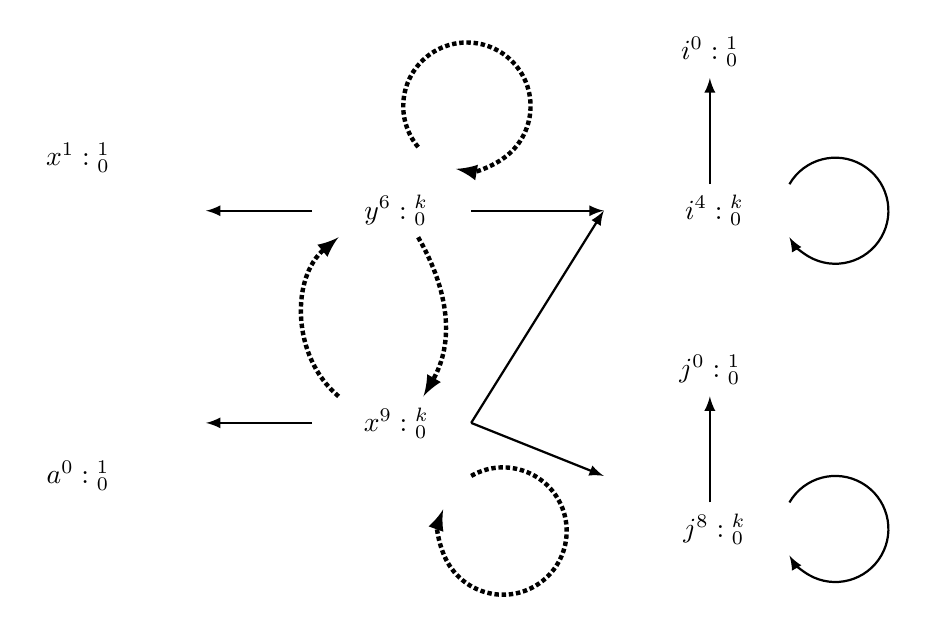
\begin{tikzpicture}[scale=\textwidth/18cm,samples=200]
% Variables Initialization
\draw[] (-6, 1) circle (0pt) node{{ $a^0: {}^1_{0}$}};
\draw[] (-6, 7) circle (0pt) node{{ $x^1: {}^{1}_{0}$}};
% Variables Inside the Loop
   \draw[] (0, 6) circle (0pt) node{{ $y^6: {}^{k}_{0}$}};
   \draw[] (0, 2) circle (0pt) node{{ $x^9: {}^{k}_{0}$}};
   % Counter Variables
   \draw[] (6, 9) circle (0pt) node {{$i^0: {}^{1}_{0}$}};
   \draw[] (6, 6) circle (0pt) node {{ $i^4: {}^{k}_{0}$}};
   \draw[] (6, 3) circle (0pt) node {{$j^0: {}^{1}_{0}$}};
   \draw[] (6, 0) circle (0pt) node {{ $j^8: {}^{k}_{0}$}};
   %
   % Value Dependency Edges:
   \draw[ ultra thick, -latex, densely dotted,] (0.5, 7.2) arc (220:-100:1.2);
   \draw[ thick, -latex] (6, 6.5)  -- (6, 8.5) ;
   \draw[ thick, -latex] (6, 0.5)  -- (6, 2.5) ;
   \draw[ ultra thick, -latex, densely dotted,] (1.5, 1.0) arc (120:-200:1.2);
   % Value Dependency Edges on Initial Values:
   \draw[ thick, -latex,] (-1.5, 2)  -- (-3.5, 2) ;
   \draw[ thick, -latex,] (-1.5, 6)  -- (-3.5, 6) ;
   %
   \draw[ ultra thick, -latex, densely dotted,] (-1, 2.5)  to  [out=-220,in=220]  (-1, 5.5);
   \draw[ ultra thick, -latex, densely dotted,]  (0.5, 5.5) to  [out=-60,in=60] (0.6, 2.5) ;
   % Control Dependency
  %  \draw[ thick,-latex] (1.5, 7)  -- (4, 9) ;
  %  \draw[ thick,-latex] (1.5, 4)  -- (4, 9) ;
  \draw[ thick, -latex, ] (7.5, 6.5) arc (150:-150:1);
  \draw[ thick, -latex, ] (7.5, 0.5) arc (150:-150:1);
  \draw[ thick,-latex] (1.5, 6)  -- (4, 6) ;
   \draw[ thick,-latex] (1.5, 2)  -- (4, 6) ;
   \draw[ thick,-latex] (1.5, 2)  -- (4, 1) ;
   \end{tikzpicture}
   \caption{}
      \end{centering}
      \end{subfigure}
    }
    % \end{wrapfigure}
    % \end{equation*}
    \vspace{-0.4cm}
     \caption{(a) The nested while loop example, (b) The program-based dependency graph generated from $\THESYSTEM$.}
    \label{fig:alg_adaptsearch_nestedwhile}
    \vspace{-0.7cm}
    \end{figure}
    %
        \begin{algorithm}
          \caption{
          {Over-Approximated Adaptivity on SCC}
          \label{alg:overadp_alg}
          }
          \begin{algorithmic}[1]
          \REQUIRE $G = (\vertxs, \edges, \weights, \qflag)$ \#\{An Strong Connected Symbolic Weighted Directed Graph\}
          % with a start vertex $s$ and destination vertex $t$ .
          \STATE {\bf {$\kw{\pathsearch_{scc-naive}(G)}$}:}  
          \STATE {\bf init} 
          \\
          $\kw{r_{scc}}$: the Adaptivity of this SCC
          \STATE  {\bf for} every vertex $v$ in $\vertxs$:
          % \STATE  \qquad initialize \kw{visited} with $\efalse$.
          \STATE  \qquad $r_{scc} += \weights(v)*\qflag(v)$  
          \RETURN $r[c]$
          \end{algorithmic}
          \end{algorithm}
          %
\begin{thm}[Soundness of $\pathsearch$]
    \label{thm:sound_adaptalg}
    For every program $c$, given its \emph{Program-Based Dependency Graph} $\progG$,
     $$\pathsearch(\progG) \geq \progA(\progG).$$
\end{thm}